\documentclass[notoc, nobib]{tufte-handout}


\usepackage{ifluatex, ifxetex} % проверка, как компилируется файл
% black magic!
% solving problem with tufte-handout + xelatex
% http://tex.stackexchange.com/questions/200722/
% https://tex.stackexchange.com/questions/47576/
\ifx\ifxetex\ifluatex\else % если xelatex или lualatex
  \newcommand{\textls}[2][5]{%
    \begingroup\addfontfeatures{LetterSpace=#1}#2\endgroup
  }
  \renewcommand{\allcapsspacing}[1]{\textls[15]{#1}}
  \renewcommand{\smallcapsspacing}[1]{\textls[10]{#1}}
  \renewcommand{\allcaps}[1]{\textls[15]{\MakeTextUppercase{#1}}}
  \renewcommand{\smallcaps}[1]{\smallcapsspacing{\scshape\MakeTextLowercase{#1}}}
  \renewcommand{\textsc}[1]{\smallcapsspacing{\textsmallcaps{#1}}}
\fi

% с альтернативного источника:
%\ifluatex % Allow rendering with LuaTeX by setting up the spacing using fontspec features
%  \renewcommand\allcapsspacing[1]{{\addfontfeature{LetterSpace=15}#1}}
%  \renewcommand\smallcapsspacing[1]{{\addfontfeature{LetterSpace=10}#1}}
%\fi

% lua produces strange notes
% https://tex.stackexchange.com/questions/328431

\usepackage{fontspec} % работа со шрифтами
%\usepackage{polyglossia} % учим русский как иностранный :)

%\setmainlanguage{engish}
%\setotherlanguages{english}

% заменяем --- на тире, << на кавычки и т.д.:
\defaultfontfeatures{Ligatures=TeX}

% download "Linux Libertine" fonts:
% http://www.linuxlibertine.org/index.php?id=91&L=1
\setmainfont{Linux Libertine O} % or Helvetica, Arial, Cambria
% why do we need \newfontfamily:
% http://tex.stackexchange.com/questions/91507/
\newfontfamily{\cyrillicfonttt}{Linux Libertine O}
\newfontfamily{\cyrillicfont}{Linux Libertine O}
\newfontfamily{\cyrillicfontsf}{Linux Libertine O}



\usepackage{amsmath}
\usepackage{amsthm}
\usepackage{amsfonts}
\usepackage{amssymb}
\usepackage{url} % вставка \url{}
\usepackage{graphicx} % вставка графиков
\usepackage{csquotes} % адаптирующиеся кавычки командой \enquote{}
\usepackage{comment} % ingore everything between \begin{comment} \end{comment}
\usepackage{answers} % separate problems and solutions
\usepackage{tikz} % pictures with tikz language
\usepackage{todonotes} % todo in documents
\usepackage{multicol} % make several columns
\usepackage{subfigure}
\usepackage{enumitem} % для создания своих нумерующих списков (хак для гиперссылок)
%\usepackage[left=2cm,right=2cm,top=2cm,bottom=2cm]{geometry}


% very useful during de-bugging!
% \usepackage[left]{showlabels}
% \showlabels{hypertarget}
% \showlabels{hyperlink}


\DeclareMathOperator{\sign}{sign}
\DeclareMathOperator{\diag}{diag}
\DeclareMathOperator{\Var}{Var}
\DeclareMathOperator{\sVar}{sVar}
\DeclareMathOperator{\pVar}{pVar}
\DeclareMathOperator{\card}{card}
\DeclareMathOperator{\Cov}{Cov}
\DeclareMathOperator{\Corr}{Corr}
\DeclareMathOperator{\sCov}{sCov}
\DeclareMathOperator{\pCov}{pCov}
\DeclareMathOperator{\sCorr}{sCorr}
\DeclareMathOperator{\pCorr}{pCorr}
\DeclareMathOperator{\E}{E}
\DeclareMathOperator{\ctg}{ctg}
\DeclareMathOperator{\tg}{tg}
\DeclareMathOperator{\Lin}{Lin}
\DeclareMathOperator{\col}{col}
\renewcommand{\P}{\mathbb{P}}
\newcommand{\I}{\mathbb{I}} % индикатор события

\newtheorem{theorem}{Theorem}
\newtheorem{corollary}{Corollary}[theorem]
\newtheorem{lemma}[theorem]{Lemma}
\theoremstyle{definition}
\newtheorem{definition}{Definition}



\usepackage[bibencoding = auto, backend = biber,
sorting = none]{biblatex}

\addbibresource{references.bib}



\title{How Gauss and Markov met Pythagoras: geometry in econometrics}
\author{Boris Demeshev\thanks{boris.demeshev@gmail.com}, Olga Gnilova\thanks{olyagnilova@gmail.com}}
%\date{\today}
\bibliography{references}
\begin{document}

\maketitle
\tableofcontents

\newpage
\section{Introduction}

\begin{fullwidth}

Pursuing abstractness and generality, a number of books and articles in
econometrics rely heavily on standard algebraic proofs.
However, most of the theorems proved in such a way have a strong geometric appeal.
The aim of this paper is to demonstrate how intuitive and elegant the proofs
can be when they are based on well-known geometric facts.
Moreover, we show that the geometric approach can be extended to explain
the concepts in probabily and statistics.

Although most of the theorems and ideas are not completely new and
there are even a few works on the geometry in econometrics and statistics,
this paper introduces alternative explanations and more general results in some cases.
Besides, there are algebraic proofs provided parallel to geometric ones
as well as illustrations which are our own work. 
The illustrations are published at \url{https://github.com/olyagnilova/gauss-markov-pythagoras} and licensed under the
Creative Commons Attribution 4.0. % todo: wiki
They are free to use and have potential to serve as a pedagogical tool
in explaining material for students.

While preparing the paper we found several works that were useful and relevant.
In particular, \citeauthor{jacobson}'s (\citeyear{jacobson}) thesis \citetitle{jacobson}
is a comprehensive overview of geometric approach in linear models including
statistical foundations.
\citeauthor{gmt_blue}’s (\citeyear{gmt_blue}) text \citetitle{gmt_blue} and
\citetitle{gmt_american_statistician} by
\citeauthor{gmt_american_statistician} (\citeyear{gmt_american_statistician}) were especially helpful when thinking over
the alternative way of proving this central theorem of econometrics.
The works that deepened our understanding of instrumental variables were
\citeauthor{Butler2016}'s (\citeyear{Butler2016}) \citetitle{Butler2016}
and \href{http://web.hku.hk/~pingyu/6005/6005.htm}{lecture notes} on Econometric theory I course by Ping Yu.
The first work that proves the Frisch-Waugh-Lovell theorem using pure geometry
is \citetitle{fwl} by
\citeauthor{fwl} (\citeyear{fwl}).
Finally, there were several works that apply the geometric approach to
hypothesis testing. They are
\citetitle{Langsrud2004}
by \citeauthor{Langsrud2004} (\citeyear{Langsrud2004}),
\citetitle{Siniksaran2005}
by \citeauthor{Siniksaran2005} (\citeyear{Siniksaran2005}),
and the one which uses an outstanding approach —
\citetitle{friendly2013}
by \citeauthor{friendly2013} (\citeyear{friendly2013}).

The paper consists of four parts. In the first one the fundamentls of the geometry
of random variables are introduced as well as examples.
In the part two, we develop the ideas related to the linear regression
from the ones which need almost no assumptions to the more sophisticated theorems
and concepts.
The next part is devoted to partial correlation. It contains a proof of
a newly-introduced fact about the partial correlation and the correlation
between the residuals in linear regression model.
Finally, the probabily distributions are introduced from the geometric perspective
and the corresponding tests are illustrated.

\end{fullwidth}


\newpage
\section{Geometric interpretation of random variables}\label{rvs}

The fundamental part to start with is defining the geometric properties of random
variables using some concepts of linear algebra.

Consider the vector space which consists of all random variables with finite
mean and variance.
We will regard each point in this space (or vector that correponds to that point
in terms of linear algebra) a random variable.
We define the scalar product of two random variables $X$ and $Y$ to be
\[
\langle X, Y \rangle = \Cov(X,Y).
\]
It is of no difficulty to check that the definition satisfies the properties
of scalar product assuming that $X$ and $Y$ are the same random variables
if $\P(X=Y)=1$.

\begin{marginfigure}
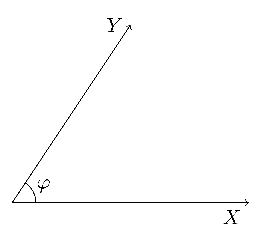
\includegraphics{figures/01_corr_def.pdf}
\caption{Geometric representation of random variables.}
\label{fig:corr_def}
\end{marginfigure}

Having defined the inner product, we are now able to introduce the squared
length of a random variable $X$ which is
\[
\lVert X \rVert^2 = \langle X, X \rangle = \Cov(X,X) = \Var(X),
\]
so the length is simply the square root of this expression, i.e., the~standard
deviation of $X$ ($\sigma_X$).

Recall that for any non-random vectors $a$ and $b$ the angle
between them is calculated with the formula
\[
\cos(a, b) = \frac{\langle a,  a\rangle}{|a| |b|}.
\]
The same applies for the random variables and it is already clear that
two random variables are uncorrelated if and only if their scalar product
equals $0$. Additionally, it means that these two random variables
are orthogonal in the vector space.

The analogue for $cos(a, b)$ in the vector space of all the random
variables is the correlation between two of them:
\[
\Corr(X,Y) = \frac{\Cov(X,Y)}{\sqrt{\Var(X)\Var(Y)}} = \frac{\langle X, Y \rangle}{\sqrt{\lVert X \rVert^2 \lVert Y \rVert^2}}.
\]
From the equivalence of $\Corr(X,Y)$ to the $\cos(a, b)$ it
automatically follows that the correlation coefficient can range from $-1$ to $1$.

\begin{marginfigure}[10\baselineskip]
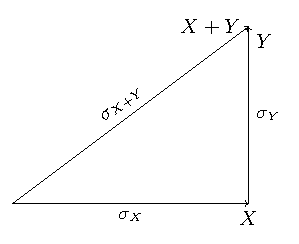
\includegraphics{figures/01_pythagorean_theorem.pdf}
\caption{The Pythagorean theorem for random variables $X$ and $Y$.}
\label{fig:rv_pyth}
\end{marginfigure}

A useful property of the geoemtry of random variables is that all the
geometric theorems still hold. For instance, the Pythagorean theorem can
be formulated as follows: if the ranadom variables $X$ and $Y$ are uncorrelated
(which implies that they are orthogonal), then the variance of their sum equals
the sum of their variances:
\[
\Var(X + Y) = \sigma^2_{X+Y} = \sigma^2_{X} + \sigma^2_{Y} = \Var(X) + \Var(Y).
\]
Translated to the non-random language, assumption of uncorrelatedness correspnds
to the right triangle setting, the variance of the sum of two random variables
stands for the hypotenuse squared and the sum of the variances is the sum of
the legs squared.

Another important geometric tool is projection.
Recall that for any two vectors the scalar product $\langle a, b \rangle$
can be interpreted as the length of projected $b$ multiplied by the length of $a$.
The projection itself is $\cos(a, b) b$.
Same holds for the random variables.
The projection of such a random variable $Y$ onto $\{cX| c \in \mathbb{R}\}$ is
$\hat Y = \Corr(X,Y) \cdot Y$.

\begin{marginfigure}
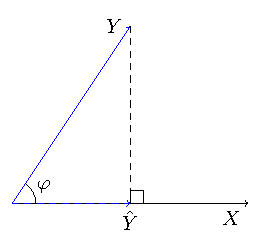
\includegraphics{figures/01_basic_projection.pdf}
\caption{The projection of a random variable $Y$ onto the line spanned by
a random varibale $X$.}
\label{fig:rv_proj}
\end{marginfigure}

Note that the squared lengths of the leg adjacent to $\varphi$ and the
hypotenuse are $\Var(\hat Y)$ and $\Var(Y)$.
So, the Figure~\ref{fig:rv_proj} gives a useful expression for the correlation
coefficient squared:
\[
\Corr^2(X,Y) = \frac{\Var(\hat Y)}{\Var(Y)}.
\]

\subsection{The law of iterated expectations}

\marginnote{
Here is the proof for the case when $X$ and $Y$ are both discrete. Let $\E(Y|X) = g(X)$.
\begin{align*}
&\E(g(X)) = \sum_x g(x) \P(X=x) \\
&= \sum_x \left( \sum_y y \P(Y=y|X=x) \right) \P(X=x) \\
&= \sum_x \sum_y y  \P(X=x) \P(Y=y|X=x)  \\
&= \sum_y y \sum_x \P(X=x, Y=y) \\
&= \sum_y y \P(Y=y) = \E(Y)
\end{align*}
The proof in case of continous random variables is absolutely analogous.
}

\begin{theorem}
For any random variable $X$ and $Y$,
\[
\E(\E(X|Y)) = \E(Y).
\]
\end{theorem}

\begin{proof}

Consider a vector space of all the random variables.  The random variables
which can be described as functions of $X$ form a subspace of that vector
space, represented as a plane $\alpha$ in Figure~\ref{fig:adams}.
Another subspace is a subspace of constants, denoted as a vector $\mathbf{1} \in \alpha$.

In order to obtain $\E(Y|X)$, first, we need to project $Y$ onto the subspace
of all the functions of $X$. As a result of this step, we get $\E(Y|X)$ — the function
of $X$ that predicts $Y$ the best (the function which gives the lowest MSE).
Next, projecting $\E(Y|X)$ onto the space of all constants, we obtain $E(Y)$.

Notice that the vector $Y - \E(Y|X)$ (which is also called the residual) is
perpendicular to the plane $\alpha$. Particularly, the vecotr $\E(Y|X) - E(Y)$ is
perpendicular to the vector of constants $\mathbf{1}$. Thus, we can apply
the theorem of three perpendiculars and conclude that the vector $Y - \E(Y)$ is
also perpendicular to the vector of constants $\mathbf{1}$.

So, we showed that the expectation of the random variable $Y$ can be obtained either
in two steps or by its direct projection onto the subpace of constans.

\begin{figure}[h!]
\begin{center}
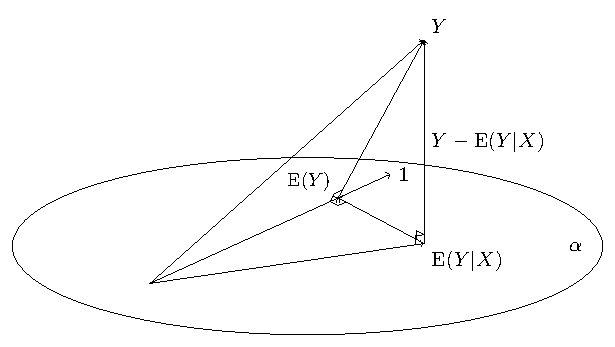
\includegraphics[width=0.6\linewidth]{figures/01_law_of_iterated_expectations.pdf}
\caption{The law of iterated expectations. Equivalence of the two-step projecttion
and direct projection of $Y$ onto $\mathbf{1}$.}
\label{fig:adams}
\end{center}
\end{figure}

\end{proof}


\subsection{MSE decomposition}

\begin{theorem}
The mean squared error of an estimator $\hat \theta$ with respect to an unknown
parameter $\theta$ defined as $MSE(\hat \theta) = \E((\hat \theta - \theta)^2)$
can be decomposed into the sum of the variance of the estimator and its squared bias:
\[
MSE(\hat \theta) = \Var(\hat \theta) + \E \left[\left( \E(\hat \theta) - \theta  \right)^2 \right]
\]
\end{theorem}

\marginnote{
\begin{align*}
&MSE(\hat \theta) = \E((\hat \theta - \theta)^2) \\
&= \E \left[ \left( \hat \theta - \E(\hat \theta) +  \E(\hat \theta) - \theta \right)^2 \right] \\
&= \E \left[ \left( \hat \theta - \E(\hat \theta) \right)^2 + 2  (\hat \theta - \E(\hat \theta)) (\E(\hat \theta) - \theta )  \right. \\
&+ \left. \left( \E(\hat \theta) - \theta  \right)^2 \right] \\
&= \E \left[\left( \hat \theta - \E(\hat \theta) \right)^2 \right] + 2 \E (\hat \theta - \E(\hat \theta)) (\E(\hat \theta) - \theta ) \\
&+ \E \left[\left( \E(\hat \theta) - \theta  \right)^2 \right] \\
&= \E \left[\left( \hat \theta - \E(\hat \theta) \right)^2 \right] \\
&+ 2 \E(\hat \theta - \E(\hat \theta)) \E(\hat \theta - \E(\hat \theta)) \\
&+ \E \left[\left( \E(\hat \theta) - \theta  \right)^2 \right] \\
&= \E \left[\left( \hat \theta - \E(\hat \theta) \right)^2 \right] + \E \left[\left( \E(\hat \theta) - \theta  \right)^2 \right] \\
&= \Var(\hat \theta) + \E \left[\left( \E(\hat \theta) - \theta  \right)^2 \right]
\end{align*}
}

\begin{proof}
We start with a random variable $\theta$ and its estimate $\hat \theta$ in the
vector space. We know that an unbiased estimator's projection would be exactly
the vector representing $\theta$. However, in general it does not have to and
Figure~\ref{fig:mse_decomposed} illustrates this case: the projection of the estimator falls onto
the line spanned by the vector $\theta$.

Connecting vectors $\theta$ and $\hat \theta$, we obtain the right triangle which
legs are $\hat \theta - \E(\hat\theta)$, $\E(\hat\theta) - \theta$ and the
hypotenuse $\hat \theta - \theta$.
Applying the Pythagorean theorem, we finish the proof:
\begin{align*}
\lVert \hat \theta - \theta \rVert^2 &= \lVert \hat \theta - \E(\hat \theta) \rVert^2  + \lVert \E(\hat \theta) - \theta \rVert^2 \\
\E((\hat \theta - \theta)^2) &= \E((\hat \theta - \E(\hat \theta))^2) + \E((\E(\hat \theta) - \theta)^2) \\
MSE(\hat \theta) &= \Var(\hat \theta) + \E((\E(\hat \theta) - \theta)^2)
\end{align*}

\begin{figure}[h!]
\begin{center}
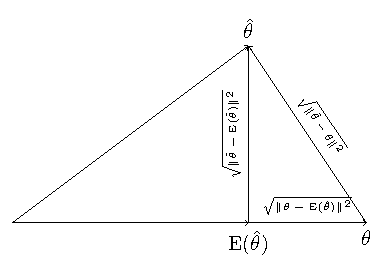
\includegraphics[width=0.6\linewidth]{figures/01_mse_decomposition.pdf}
\caption{Decomposition of mean squred error into the variance and the bias squared
$\left(a = \sqrt{\lVert\hat\theta - \E(\hat\theta)\rVert^2} \right.$, $b = \sqrt{\lVert \theta - \E(\hat\theta) \rVert^2}$, $\left. c = \sqrt{\lVert \hat\theta - \theta \rVert^2} \right)$}
\label{fig:mse_decomposed}
\setfloatalignment{b}
\end{center}
\end{figure}

\end{proof}


\newpage
\section{Regression}

The concepts discussed in the following section could also be presented in
random variables instead of sample ones. As the geometry of sample variables
is almost of no difference comparing to the random ones, the logic of
all the theorems is also the same.


\subsection{Geometry of sample variables}

\marginnote{
\begin{multline*}
\sCorr(x,y) = \frac{\sCov(x,y)}{\sqrt{\sVar(x)\sVar(y)}} \\
= \frac{\frac{1}{n-1}\sum_{i=1}^n (x_i - \bar x)(y_i - \bar y)}{\sqrt{\frac{1}{n-1} \sum_{i=1}^n (y_i - \bar y)\frac{1}{n-1} \sum_{i=1}^n (\hat y_i - \bar{\hat y})}}
\end{multline*}
}

In the~same manner it was done in the previous section, we define
the~scalar product of two sample variables
$x =
\begin{pmatrix}
x_1 \\
\vdots \\
x_n
\end{pmatrix}$
and
$y =
\begin{pmatrix}
y_1 \\
\vdots \\
y_n
\end{pmatrix}$
as a sample covariation between them:
\[
\langle x, y \rangle = \sCov(x, y).
\]
The main characteristics of a~vector are its length and direction.
Again, we introduce the~length
\[
\sqrt{\sCov(x,x)} = \sqrt{\sVar(x)} = \sigma_x
\]
and the~angle between two sample variables
\[
\cos(x,y) = \frac{\sCov(x,y)}{\sqrt{\sVar(x)\sVar(y)}} = \sCorr(x,y).
\]
Note that from the definition of the angle
it follows that the~sample correlation coefficient can range from $-1$ to $1$.

\begin{marginfigure}
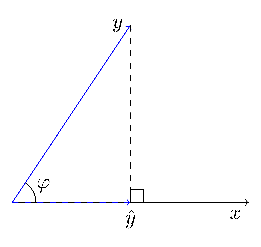
\includegraphics[scale=0.85]{figures/02_basic_projection.pdf}
\caption{Vector $y$ projected onto vector $x$.}
\label{fig:corr_proj}
\end{marginfigure}

Completely analogus to the~case of random variables,
the projection of such a sample variable $y$ onto
$\{cx| c \in \mathbb{R}\}$ is $\hat y = \sCorr(x,y) \cdot y$.

Looking at Figure~\ref{fig:corr_proj}, we can interpret the~square of sample correlation coefficient.
Using the fact that $cos^2 \varphi$ is the~squared ratio of
the~leg adjacent to $\varphi$ to hypotenuse, we can conclude that
\[
\sCorr^2(x,y) = \frac{\sVar(\hat y)}{\sVar(y)},
\]
as the variance of a vector is associated with the square of its length.
Thus, the~sample correlation coefficient squared shows
the~fraction of variance in $y$ which can be explained
with the~most similar vector proportional to $x$.


\subsection{Sample correlation when a constatnt vector added}

\marginnote{
\begin{align*}
\sCorr(x + \alpha \mathbf{1}, y) &= \frac{\sCov(x + \alpha \mathbf{1}, y)}{\sqrt{\sVar(x + \alpha \mathbf{1}) \sVar(y)}} \\
&= \frac{\sCov(x,y) + \sCov(\alpha \mathbf{1},y)}{\sqrt{\sVar(x)\sVar(y)}} \\
&= \frac{\sCov(x,y)}{\sqrt{\sVar(x)\sVar(y)}} \\
&= \sCorr(x,y)
\end{align*}
}

\begin{theorem}
Adding a~vector of constants does not affect the sample correlation coefficient:
\[
\sCorr(x + \alpha \mathbf{1}, y) = \sCorr(x,y)
\]
where $\alpha \in \mathbb{R}$.
\end{theorem}

\begin{proof}
Firstly, we project vectors $x$ and $y$ onto $\Lin^{\perp}(\mathbf{1})$
in order to get $x^c = x - \bar x$ and $y^c = y - \bar y$ (`c' stands for `centred').
It can be shown that the~matrix corresponding to projecting onto the line spanned by
a~vector of all ones has the~following form
\[
\frac{\mathbf{1}^T \mathbf{1}}{\mathbf{1} \mathbf{1}^T} = \frac{\begin{pmatrix} 1 & \ldots & 1 \end{pmatrix} \begin{pmatrix} 1 \\ \vdots \\ 1 \end{pmatrix}}{\sum_{i=1}^n 1} = \begin{pmatrix} \frac{1}{n} & \ldots & \frac{1}{n} \\ \vdots & \ddots & \vdots \\ \frac{1}{n} & \ldots & \frac{1}{n} \end{pmatrix}
\]
Thus, projecting onto the~orthogonal subspace is equivalent to
substracting the~projected vector, i.e., the vector of averages, from the original one.

\begin{marginfigure}
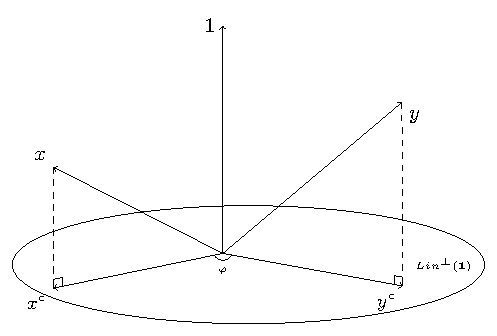
\includegraphics[scale=0.65]{figures/02_correlation_constant_centered_variables.pdf}
\caption{Centred vectors $x^c$ and $y^c$}
\label{fig:corr_xyc}
\end{marginfigure}

Also note that the~angle $\varphi$ between the~original and centred vectors remains the~same.
The~result of this step is shown in Figure~\ref{fig:corr_xyc}.

Then we need to derive a new vector $\tilde x$ with constants added to each component.
Geometrically adding a vector of costants means adding a vector of all ones
scaled by $\alpha \in \mathbb{R}$, i.e., $\alpha \mathbf{1}$.
Then the new vector $\tilde x$ can be broken up into a sum of $\alpha \mathbf{1}$ and
$\beta x$, $\alpha, \beta \in \mathbb{R}$, which can be seen in Figure~\ref{fig:corr_final}.
After that we will project this new vector $\tilde x$ onto $\Lin^{\perp}(\mathbf{1})$.
By the properties of projection it is of no difference whether to project
the whole vector $\tilde x$ or project its parts $\alpha \mathbf{1}$
and $\beta x$ — the result is the same.
So, while $\beta x$ is projected onto the span of $x^c$, the projection of $\alpha \mathbf{1}$
onto the orthohgonal space $\Lin^{\perp}(\mathbf{1})$ yields zero as demonstrated
in Figure~\ref{fig:corr_final}.
Moreover, it follows that the angle between $\tilde x$ and $y$ is still $\varphi$.

\begin{figure}
\begin{center}
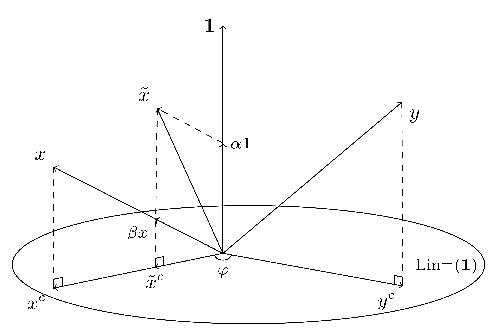
\includegraphics[width=0.6\linewidth]{figures/02_correlation_constant_proof.pdf}
\label{fig:corr_final}
\caption{$\sCorr(x + \alpha \mathbf{1}, y) = \sCorr(x,y)$ as the corresponding angles are equal..}
\end{center}
\end{figure}


Finally, putting everything together we finish the proof:
\[
\sCorr(x + \alpha \mathbf{1}, y) = \sCorr(x,y)
\]
\end{proof}


\subsection{Sample correlation coefficient in simple linear regression}

\begin{theorem}
A linear regression model with one explanatory variable and constant term
\[
y = \beta_1 + \beta_2 x + \varepsilon
\]
has the property
\[
\sCorr(y, \hat y) = sign(\hat \beta_2) \sCorr(y, x)
\]
\end{theorem}

\marginnote{
Assuming the underlying relationship between $x$ and $y$ to be
\[
y_i = \beta_1 + \beta_2 x_i + \varepsilon_i \quad i=1,\ldots,n
\]
where $\varepsilon_i$ is an error term the following holds
\begin{align*}
\sCorr(y, \hat y) &= \frac{\sCov(y, \hat y)}{\sqrt{\sVar(y)\sVar(\hat y)}} \\
&= \frac{\sCov(y, \hat \beta_1 + \hat \beta_2 x)}{\sqrt{\sVar(y)\sVar(\hat \beta_1 + \hat \beta_2 x)}} \\
&= \frac{\sCov(y, \hat \beta_2 x)}{\sqrt{\sVar(y)\sVar(\hat \beta_2 x)}} \\
&= \frac{\hat \beta_2 \sCov(y, x)}{|\hat \beta_2| \sqrt{\sVar(y)\sVar(x)}} \\
&= sign(\hat \beta_2) \frac{\sCov(y,x)}{\sqrt{\sVar(y)\sVar(x)}} \\
&= sign(\hat \beta_2) \sCorr(y, x)
\end{align*}
}

\begin{proof}
Firstly, we consider the case when $\hat \beta_2 > 0$.
It has been shown earlier that the correlation coefficient represents the angle
between two random vectors.
So, in order to complete the proof we need to find the appropriate angles and compare them.

However, it seems to be difficult to compare the angles in the three dimensional space.
That is why we start with projecting both $x$ and $y$ onto the plane perpendicular to the vector of all ones (denoted as $\mathbf{1}$) as shown in Figure~\ref{fig:corr_pos_xyc}.
We denote this space as $\Lin^{\perp}(\mathbf{1})$. The resulting vectors are $x - \bar x \cdot \mathbf{1}$  and $y - \bar y \cdot \mathbf{1}$, respectively,
since projection of any vector $\vec{a}$ onto the span of a vector of all ones yields the vector of averages $\vec{\bar a}$.


In order to get the angle between $y$ and $\hat y$ we should start with regressing $y$ on $\Lin(x, \mathbf{1})$.
Then the only thing left is to project $\hat y$ onto $\Lin^{\perp}(\mathbf{1})$ since the $y$ vector has already been projected.
Note that the projected $\hat y$ falls onto tha span of vector $x - \bar x \cdot \mathbf{1}$ as it can be decomposed into a sum $a x + b \mathbf{1}$ where $a, b \in \mathbb{R}$.
The first component $a x$ is projected in the same way as $x$ and $b \mathbf{1}$ yields zero when projected onto the orthogonal space.
The result of this step is shown in Figure~\ref{fig:corr_pos_yhatc}.

\begin{figure*}[h!]
\begin{center}
\subfigure[]{
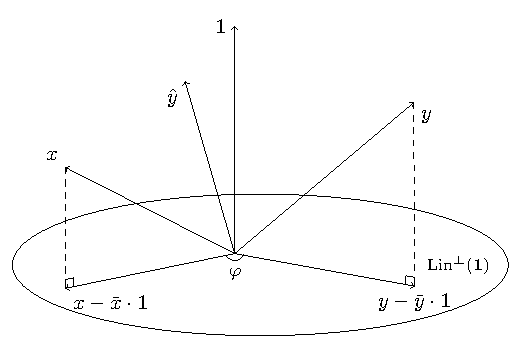
\includegraphics[width=0.45\linewidth]{figures/02_simple_regression_coefficient_centred_variables.pdf}
\label{fig:corr_pos_xyc}}
%\hspace{4ex}
\subfigure[]{
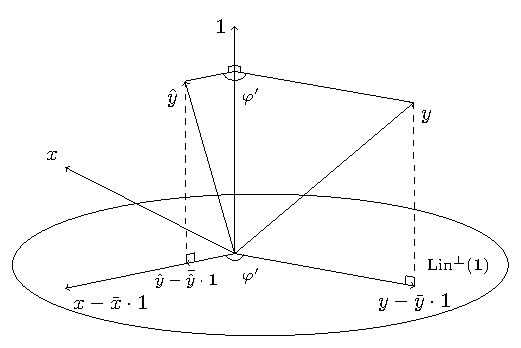
\includegraphics[width=0.45\linewidth]{figures/02_simple_regression_coefficient_yhat_projected.pdf}
\label{fig:corr_pos_yhatc}}
\caption{\subref{fig:corr_pos_xyc}: `Centred' $x$ and $y$, i.e., projected onto $\Lin^{\perp}(\mathbf{1})$; \subref{fig:corr_pos_yhatc}: `Centred' $\hat y$, i.e., projected onto $\Lin^{\perp}(\mathbf{1})$.}
\end{center}
\end{figure*}

Since the projection of $\hat y$ lies exactly on the span of vector $x - \bar x \cdot \mathbf{1}$, we can conclude that $cos \varphi = \cos \varphi '$ and to put it another way $\sCorr(x,y) = \sCorr(y, \hat y)$.

Now consider the case when $\hat \beta_2 < 0$.
Note that the sign of $\beta_1$ does not influence the correlation coefficient sign.
The only difference is that now $\hat y$ is projected onto the span of  $x - \bar x \cdot \mathbf{1}$ and not on this vector itself while the projections of $x$ and $y$ remain the same.
Looking at Figure~\ref{fig:corr_negative} we deduce
that the~angle between $y$ and $\hat y$ is compelement to the angle between $x$ and $y$.
Using trigonometric properties, we simplify $\cos(180^{\circ} - \varphi) = -\cos\varphi$
which in turn implies $\sCorr(x,y) = -\sCorr(y,\hat y)$.

\begin{figure}[h!]
\begin{center}
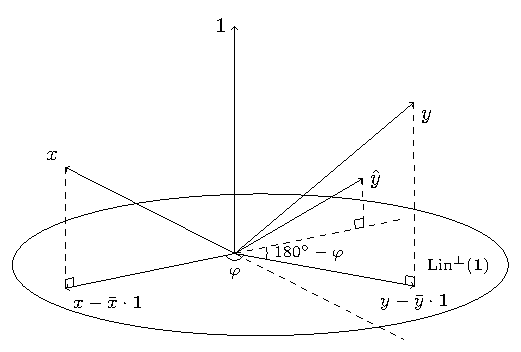
\includegraphics{figures/02_simple_regression_coefficient_negative.pdf}
\label{fig:corr_negative}
\caption{Case of $\beta_2 < 0$.}
\setfloatalignment{b}
\end{center}
\end{figure}
\end{proof}


\subsection{RSS + ESS = TSS}

\marginnote{
Consider a regression model with $n$ observations and $k$ explanatory variables
including a constant unit vector % unit?
\[
y = X \beta + \varepsilon
\]
The OLS estimator for the vector of coefficients $\beta$ is
\[
\hat \beta = (X^T X)^{-1} X^T y
\]
and the residual vector is
\begin{align*}
\hat e &= y - \hat y \\
&= y - X \hat \beta \\
&= y - X (X^T X)^{-1} X^T y
\end{align*}
Then we define residual sum of squares (RSS), explained sum of squares (ESS) and total sum of squares (TSS) as follows:
\begin{align*}
RSS &= \lVert y - \hat y \rVert^2_2 \\
ESS &= \lVert \hat y - \bar y \rVert^2_2 \\
TSS &= \lVert y - \bar y \rVert^2_2 \\
\end{align*}
}

\begin{theorem}
A linear regression model with $n$ observations and $k$ explanatory variables including a constant unit vector
\[
y = X \beta + \varepsilon
\]
has the following property
\[
RSS + ESS = TSS
\]
where $RSS = \lVert y - \hat y \rVert^2_2$, $ESS = \lVert \hat y - \bar y \rVert^2_2$, $TSS = \lVert y - \bar y \rVert^2_2$.
\end{theorem}

\begin{proof}
The proof will be presented for the case of two regressor $x$ and $\mathbf{1}$ in order for the picture to be clear.
However, the same logic applies for the case of $k$ regressors.

We start with depicting the vectors $y \in \mathbb{R}^{n-2}$ and $x, \mathbf{1} \in \mathbb{R}^2$.
Then we project $y$ onto $\Lin(x, \mathbf{1})$ and obtain $\hat y$ which is shown in Figure~\ref{fig:rss}.

From this picture we can immediately derive $\sqrt{RSS}$ as by definition this is the squared difference between $y$ and $\hat y$.

\begin{figure*}[h!]
\begin{center}
\subfigure[]{
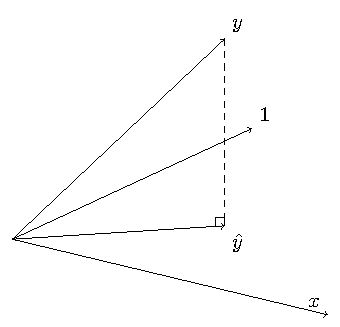
\includegraphics[width=0.3\linewidth]{figures/02_rss_ess_tss_yhat.pdf}
\label{fig:rss}}
\hspace{4ex}
\subfigure[]{
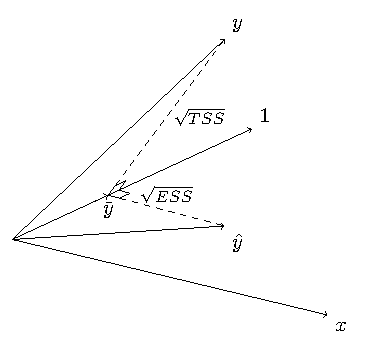
\includegraphics[width=0.3\linewidth]{figures/02_rss_ess_tss_sqr_tss_ess.pdf}
\label{fig:tss_ess}}
\subfigure[]{
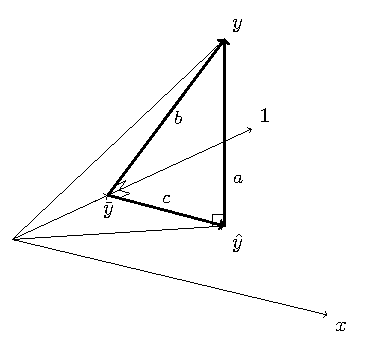
\includegraphics[width=0.3\linewidth]{figures/02_rss_ess_tss_final.pdf}
\label{fig:final}
}
\caption{\subref{fig:rss}: Residual sum of squares;
\subref{fig:tss_ess}: Total sum of squares and residual sum of squares;
\subref{fig:final}: Illustration of the equality $(\sqrt{RSS})^2 + (\sqrt{ESS})^2 = (\sqrt{TSS})^2$
where $a$ stands for $\sqrt{RSS}$, $b$ — $\sqrt{TSS}$, $c$ — $\sqrt{ESS}$.}
\end{center}
\end{figure*}

So as to visualize $ESS$ and $TSS$ we first need to visualize vector of averages $\bar y$.
Geometrically this means projecting a vector onto a line spanned by vector $\mathbf{1}$.

Now we both project $y$ and $\hat y$ onto $\mathbf{1}$ and following the definition obtain $\sqrt{TSS}$ as the difference vector $y - \bar y$ and $\sqrt{ESS}$ as the vector $\hat y - \bar y$.

The final step is to put everything together.
Note that since $y - \hat y$ is perpendicular to $\Lin(x, \mathbf{1})$ it is also perpendicular to $\hat y - \bar y$ and $\mathbf{1}$ as these vectoros are in $\Lin(x, \mathbf{1})$.
Then, applying the theorem of three perpendiculars we conclude that the foot of vector $y - \bar y$ is the same point as the foot of the vector $\hat y - \bar y$.
Thus, we obtain a right angle triangle and can apply the Pythagorean theorem for the catheti $\sqrt{RSS}$ and $\sqrt{ESS}$ and the
hypotenuse $\sqrt{TSS}$:
\[
\left(\sqrt{RSS}\right)^2 + \left(\sqrt{ESS}\right)^2 = \left(\sqrt{TSS}\right)^2
\]

\marginnote[-5\baselineskip]{
Disclosing parentheses and using the fact that $\hat{y}^T y = \hat{y}^T \hat{y}$
\begin{align*}
\hat{y}^T y &= \beta^T X^T y \\
&=  y^T X (X^T X)^{-1} X^T y \\
\hat{y}^T \hat{y} &= \beta^T X^T X \beta \\
&= y^T X (X^T X)^{-1} X^T X (X^T X)^{-1} X^T y \\
&= y^T X (X^T X)^{-1} X^T y
\end{align*}
we obtain
\begin{align*}
RSS &= y^T y -\hat{y}^T \hat{y} \\
ESS &= \hat{y}^T \hat{y} - \hat{y}^T \bar{y} + \bar{y}^T \bar{y} \\
TSS &= y^T y - 2 y^T \bar y +  \bar{y}^T \bar{y}
\end{align*}
When putting everything together all the terms cancel out which proves
\[
ESS + RSS = TSS
\]
}
\end{proof}

\vspace{3.5cm}
\subsection{Determination coefficient}

\marginnote[-2\baselineskip]{
\begin{align*}
\sCorr^2(y,\hat y) &= \left(\frac{\sCov(y, \hat y)}{\sqrt{\sVar(y)\sVar(\hat y)}}\right)^2 \\
&= \frac{\sCov(y, \hat y) \sCov(y, \hat y)}{\sVar(y)\sVar(\hat y)} \\
&= \frac{\sCov(\hat y + e, \hat y) \sCov(\hat y + e, \hat y)}{\sVar(y)\sVar(\hat y)} \\
&= \frac{\sCov(\hat y, \hat y) + \sCov(e, \hat y)}{\sVar(y)} \\
&\cdot \frac{\sCov(\hat y, \hat y) + \sCov(e, \hat y)}{\sVar(\hat y)} \\
&= \frac{\sVar(\hat y) \sVar(\hat y)}{\sVar(y)\sVar(\hat y)} \\
&= \frac{\sVar(\hat y)}{\sVar(y)} = \frac{ESS}{TSS} = R^2
\end{align*}
}

\begin{theorem}
A linear regression model with $n$ observations and $k$ explanatory variables including a constant unit vector
\[
y = X \beta + \varepsilon
\]
has the following property
\[
R^2 = \sCorr^2(y, \hat y)
\]
\end{theorem}

\begin{proof}
Proving this theorem geometrically means showing that the determination coefficient can be interpreted as some squared angle
which happens to be eqaul to the squared angle betwen $y$ and $\hat y$.

Consider Figure~\ref{fig:final} from the previous proof.
It was shown there that the vectors $y - \bar y$, $y - \hat y$ and $\hat y - \bar y$ form a right triangle.
Having defined the determination coefficient as
\[
R^2 = \frac{ESS}{TSS}
\]
we conclude that its geometric interpretaion is
\[
R^2 = \frac{ESS}{TSS} = \cos^2 \varphi
\]
as shown in Figure~\ref{fig:r_sq_angle}.

\begin{marginfigure}
  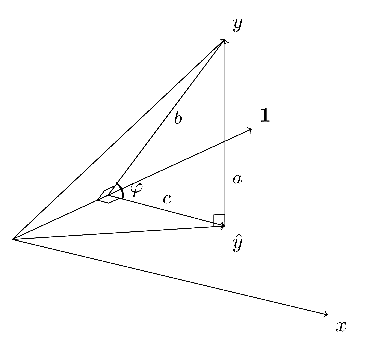
\includegraphics{figures/02_determination_coefficient.pdf}
  \caption{Determination coefficient as squared $\cos \varphi$
  where $a$ stands for $\sqrt{RSS}$, $b$ — $\sqrt{TSS}$, $c$ — $\sqrt{ESS}$}
  \label{fig:r_sq_angle}
\end{marginfigure}

Recall that the sample correlation coefficient two vectors was defined earlier as the angle between these two vectors.
Thus, we conclude that $\sCorr(y, \hat y)$ is the angle between $y$ and $\hat y$ which is also eqaul to $\cos \varphi$.
Finally, squaring both sides, we obtain
\[
R^2 = \sCorr^2(y, \hat y)
\]
\end{proof}


\subsection{Regression line and point of averages}

\marginnote[-1\baselineskip]{
If the regression contains the intercept, the following equation holds:
\begin{align*}
\hat y  &= X \hat \beta = X (X^T X)^{-1} X^T y \\
&= X (X^T X)^{-1} X^T X \beta + X (X^T X)^{-1} X^T \varepsilon
\end{align*}
Premultiplying both sides by $X^T$, we obtain:
\begin{align*}
X^T \hat y &=  X^T X (X^T X)^{-1} X^T X \beta \\
&+ X^T X (X^T X)^{-1} X^T \varepsilon \\
&= X^T X \beta + X^T \varepsilon
\end{align*}
This is a system of equations. The first row of $X^T$ is $\mathbf{1}$ vector, so we can write out the first equation:
\[
\sum_{i=1}^n \hat y_i = \sum_{i=1}^{n} \sum_{j=1}^{k} x_{ij} \beta_{j}
\]
From the first equation in the system
\[
X^T \hat y = X^T y
\]
we obtain
\[
\sum_{i=1}^{n} \hat y_i = \sum_{i=1}^{n} y
\]
And this finishes the proof:
\[
\frac{1}{n} \sum_{i=1}^{n} y = \frac{1}{n} \sum_{i=1}^{n} \sum_{j=1}^{k} x_{ij} \beta_{j}
\]
}

\begin{theorem}
In a linear regression model with one explanatory variable and constant term
\[
y = \beta_1 + \beta_2 x + \varepsilon
\]
the point of averages lies on the estimated regression line.
\end{theorem}

\begin{proof}
For the geometrical proof it suffices to show that $\hat y$ is a linear combination of the regressors, which is true by construction,
and that $\frac{1}{n} \sum_{i=1}^{n} \hat y_i = \frac{1}{n} \sum_{i=1}^{n} y$. In order for the pictures to be more clear the proof will be presented for the case of two regressors.

The first step is regressing $y$ on $\Lin(\mathbf{1}, x)$. As shown in Figure~\ref{fig:averages_lin}, we obtain $\hat y$ as a linear combination of $\mathbf{1}$ and $x$.
The next step is to regress both $y$ and $\hat y$ on $\mathbf{1}$ which results in $\bar y$ and $\bar \hat y$ correspondingly.
By the theorem of three perpendiculars, $\bar y = \bar{\hat y}$ which is shown in Figure~\ref{fig:averages_bars}.

\begin{figure}[ht!]
\begin{center}
\subfigure[]{
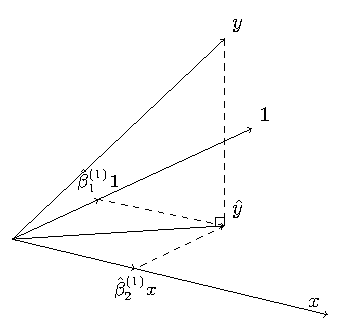
\includegraphics[width=0.35\linewidth]{figures/02_averages_yhat_decomposed.pdf}
\label{fig:averages_lin} }
\hspace{4ex}
\subfigure[]{
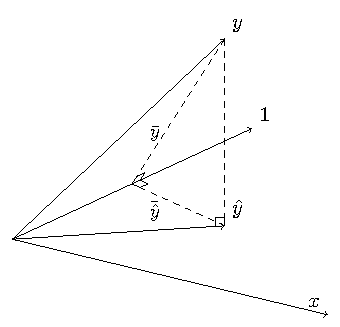
\includegraphics[width=0.35\linewidth]{figures/02_averages_final.pdf}
\label{fig:averages_bars}}
\caption{\subref{fig:averages_lin}: Regression of $y$ on $\Lin(\mathbf{1},x)$;
\subref{fig:averages_bars}: Regression of $y$ and $\hat y$ on $\mathbf{1}$.}
\setfloatalignment{b}
\end{center}
\end{figure}
\end{proof}


\subsection{Frisch–Waugh–Lovell theorem}

\marginnote{From regresison~(\ref{eq:fwl_2}) we get the following estimator:
\begin{align*}
\hat\beta_2 &= ((M_1 X_2)^T M_1 X_2)^{-1}(M_1 X_2)^T M_1 y \\
&= (X_2^T M_1^T M_1 X_2)^{-1}  X_2^T M_1^T M_1 y \\
&= (X_2^T M_1 X_2)^{-1}  X_2^T M_1 y
\end{align*}
As for regresison~(\ref{eq:fwl_1}), let us note that due to $y = \hat y + \hat u$ $y$ can be decomposed as follows:
\[
y = Py + My = X_1 \hat \beta_1 + X_2 \hat \beta_2 + My
\]
Premultiplying both sides by $X_2^T M_1$, we obtain:
\begin{align*}
X_2^T M_1 y &= X_2^T M_1 X_1 \hat\beta_1 + X_2^T M_1 X_2 \hat\beta_2 + X_2^T M_1 M y \\
&=  X_2^T M_1 X_2 \hat\beta_2 + X_2^T M_1 M y \\
&= X_2^T M_1 X_2 \hat\beta_2
\end{align*}
On the last step we used the fact that
\begin{align*}
(X_2^T M_1 M y)^T = y^T M^T M_1^T X_2 \\
= y^T M M_1 X_2 = y^T M X_2 = 0^T
\end{align*}
Assuming $X_2^T M_1 X_2$ is invertible, we get the same estimator
\[
\hat\beta_2 = (X_2^T M_1 X_2)^{-1}  X_2^T M_1 y
\]
}

\begin{theorem}
Consider regression
\begin{equation} \label{eq:fwl_1}
y = X_1 \beta_1 + X_2 \beta_2 + u
\end{equation}
where $X_{n \times k} = [X_1 X_2]$, i.e. $X_1$ consists of first $k_1$ columns of $X$ and $X_2$ consists of remaining $k_2$ columns of $X$,
$\beta_1$ and $\beta_2$ are comfortable, i.e. $k_1 \times 1$ and $k_2 \times 1$ vectors.
Consider another regresison
\begin{equation}  \label{eq:fwl_2}
M_1 y = M_1 X_2 \beta_2 + M_1 u
\end{equation}
where $M_1 = I - P_1$ projects onto the~orthogonal complement of the~column space~of
$X_1$ and $P_1 = X_1(X_1^TX_1)^{-1}X_1^T$ is the~projection onto the~column space of~$X_1$.
Then the~estimate of $\beta_2$ from regression~(\ref{eq:fwl_1}) will be the~same
as the~estimate from regression~(\ref{eq:fwl_2}).
\end{theorem}

There are two ways to~visualize the~proof of~the~Frisch-Waugh-Lovell theorem
using geometric concepts. Both are presented below.

\begin{proof}
1.~Consider the following model:
\begin{equation} \label{eq:fwl_proof}
y_i = \beta_1 x_i + \beta_2 z_i + u_i
\end{equation}

We start with a `one-step' regression  and will distinct its coefficients with
an upper index $(1)$.
The~only step in~obtaining $\beta_1^{1}$ is regressing $y$ on~$\Lin(x,z)$ and
then expanding $\hat y$ as a~linear combination of~basis vectors $x$ and $z$,
which is shown in~Figure~\ref{fig:fwl_1_regression_3d}. Figure~\ref{fig:fwl_1_regression_lin}
depicts $\Lin(x, z)$.

\begin{figure}[ht!]
\begin{center}
\subfigure[]{
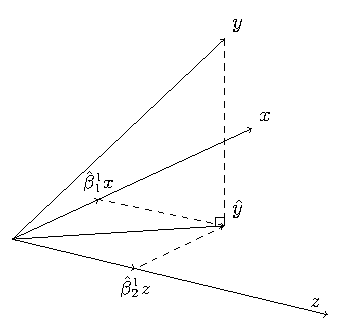
\includegraphics[width=0.4\linewidth]{figures/02_fwl_v1_yhat_decomposed.pdf}
\label{fig:fwl_1_regression_3d} }
\hspace{4ex}
\subfigure[]{
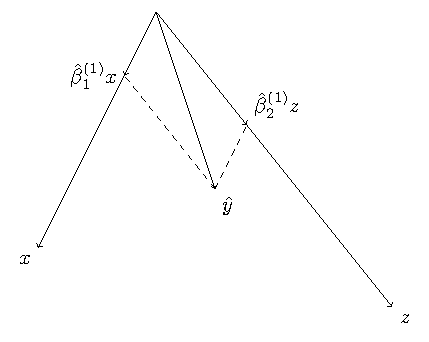
\includegraphics[width=0.4\linewidth]{figures/02_fwl_v1_yhat_decomposed_lin.pdf}
\label{fig:fwl_1_regression_lin}}
\caption{\subref{fig:fwl_1_regression_3d}: Regression of $y$ on $\Lin(x,z)$;
\subref{fig:fwl_1_regression_lin}: $\Lin(x, z)$.}
\end{center}
\end{figure}

As for the~model~(\ref{eq:fwl_2}) where several regressions are performed consecutively
we start with regressing $y$~on~$z$, resulting in $\tilde{y}$,
which we will refer~to as~`cleansed' $y$.

\begin{equation}\label{eq:fwl_2_y_clean}
\begin{aligned}
y &= \alpha z + \varepsilon \\
\hat\alpha &= \frac{y^T z}{z^T z} \\
\tilde{y} &= \hat\varepsilon = y - \frac{y^T z}{z^T z}z
\end{aligned}
\end{equation}

Following that, $x$ is regressed on $z$, resulting in $\tilde{x}$ — `cleansed' $x$.

\begin{equation}\label{eq:fwl_2_x_clean}
\begin{aligned}
x &= \gamma z + \nu \\
\hat\gamma &= \frac{x^T z}{z^T z} \\
\tilde{x} &= \hat\nu = x - \frac{x^T z}{z^T z}z
\end{aligned}
\end{equation}

Geometric results of these two steps are presented in~\ref{fig:fwl_2_regression_first}.

Finally, `cleansed' $y$ must be regressed on `cleansed' $x$.
However, it cannot be performed immediately as $\tilde{y}$ and $\tilde{x}$ are skew lines.
So at first, we fix this problem by translation and after that obtain
$\hat\beta_1^{2}\tilde x$ (see Figure~\ref{fig:fwl_2_regression_trans}).

\begin{figure}[ht!]
\begin{center}
\subfigure[]{
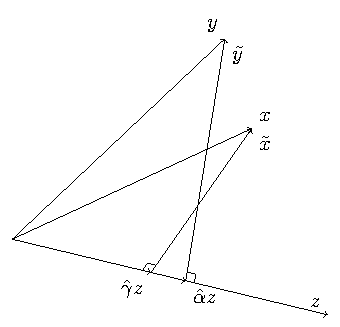
\includegraphics[width=0.4\linewidth]{figures/02_fwl_v1_cleansed_variables.pdf}
\label{fig:fwl_2_regression_first} }
\hspace{4ex}
\subfigure[]{
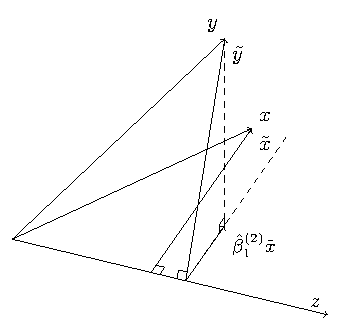
\includegraphics[width=0.4\linewidth]{figures/02_fwl_v1_translation.pdf}
\label{fig:fwl_2_regression_trans}}
\caption{\subref{fig:fwl_2_regression_first}: Regression of $y$ on $z$ and of $x$ on $z$;
\subref{fig:fwl_2_regression_trans}: Translation of $\tilde{x}$.}
\end{center}
\end{figure}

Now let us picture all the results in one figure and mark some main points.

\begin{figure}[ht!]
\begin{center}
\subfigure[]{
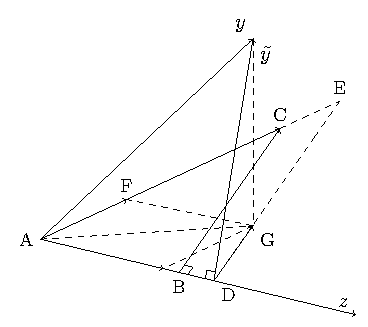
\includegraphics[width=0.4\linewidth]{figures/02_fwl_v1_final.pdf}
\label{fig:fwl_3_3d} }
\hspace{4ex}
\subfigure[]{
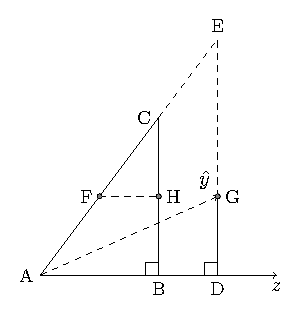
\includegraphics[width=0.4\linewidth]{figures/02_fwl_v1_final_lin.pdf}
\label{fig:fwl_3_lin}}
\caption{\subref{fig:fwl_3_3d}: Point A stands for the origin, B — $\hat\gamma z$,
C — $x$, D — $\hat\alpha z$, E — intersection of vector $x$ and line parallel to $\tilde x$,
F — $\hat\beta_1^{(1)} x$, G — $\hat\beta_1^{(2)} \tilde{x}$; \subref{fig:fwl_3_lin}: $\Lin(x,z)$.}
\end{center}
\end{figure}

In Figure~\ref{fig:fwl_3_lin} segments $AF$ and $BH = DG$ stand for $\hat\beta_1^{1}x$
and $\hat\beta_1^{2}\tilde x$ respectively, while segments AC and BC represent $x$ and $\tilde{x}$.
Having two congruent angles, triangles ABC and FHC are simillar.
Then, it follows:
\[
\frac{AF}{AC} = \frac{BH}{BC} \Leftrightarrow \frac{\hat\beta_1^{1}x}{x} = \frac{\hat\beta_1^{2}\tilde x}{\tilde x} \Leftrightarrow \hat\beta_1^{1} = \hat\beta_1^{2}
\]

2. Alternatively, we could implement a~concept close to the~partial correlation.
In the~same model~(\ref{eq:fwl_proof}) we wiil treat $z$ vector fixed and again
consecutively cleanse the $x$ and $y$ variables by projecting them onto
the~space orthogonal to $z$, i.e., $\Lin^\perp(z)$ as demonstrated in Figure~\ref{fig:fwl_v2_rcleansed}.
Then we perform a~regression of the~`cleansed' $\tilde y$ on the~`cleansed' $\tilde x$
(see Figure\ref{fig:fwl_v2_regression_cleansed}).

\begin{figure}[ht!]
\begin{center}
\subfigure[]{
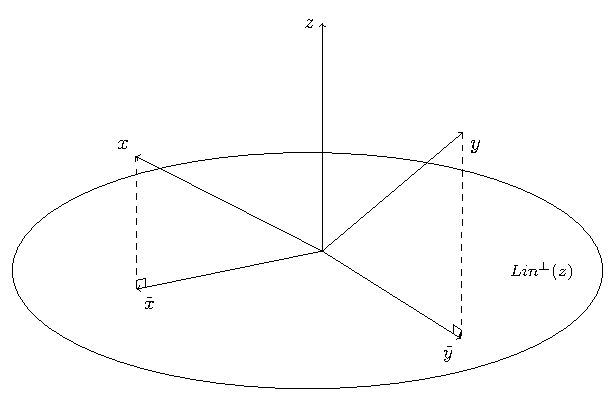
\includegraphics[width=0.45\linewidth]{figures/02_fwl_v2_cleansed_variables.pdf}
\label{fig:fwl_v2_rcleansed}}
\subfigure[]{
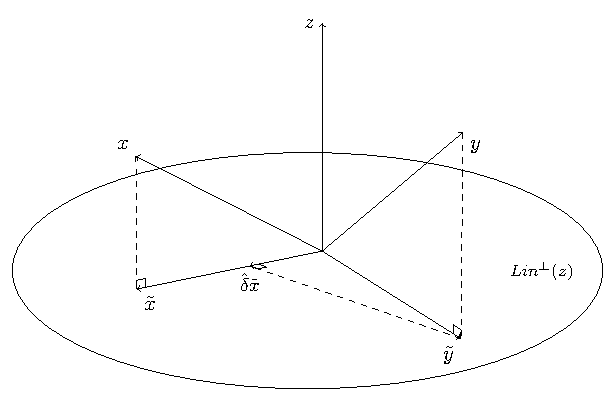
\includegraphics[width=0.45\linewidth]{figures/02_fwl_v2_cleansed_regression.pdf}
\label{fig:fwl_v2_regression_cleansed}}
\caption{\subref{fig:fwl_2_regression_first}: `Cleansed' variables $\tilde x$ and $\tilde y$;
\subref{fig:fwl_2_regression_trans}: `Cleansed' $\tilde y$ regressed on `cleansed' $\tilde{x}$.}
\end{center}
\end{figure}

Now we show that the~latter regression produces $\hat \beta_1$ coefficient which
is exactly the~coefficient from the~`one-step' regression of~original $y$ onto
original $x$ and $z$. Recall that the~vector $y$ can be split~up into a~sum of
some multiple of $x$ and some multiple of $z$. Since the second term is
the~orthogonal component its projection yields zero. The~multiple of $x$
is equal to $\hat \beta_1$ by construction.

Assume that the~coefficient at~$\tilde x$ is some unknown variable $\hat \delta$.
Then consider the~similar triangles in the $\Lin(x,z)$. From the~proportions
we obtain:
\[
\frac{CE}{CA} = \frac{CD}{CB} \Leftrightarrow \frac{\hat \beta_1 x}{x} = \frac{\hat \delta \tilde x}{\tilde x} \Rightarrow \hat \beta_1 = \hat \delta
\]

\begin{figure}[ht!]
\begin{center}
\subfigure[]{
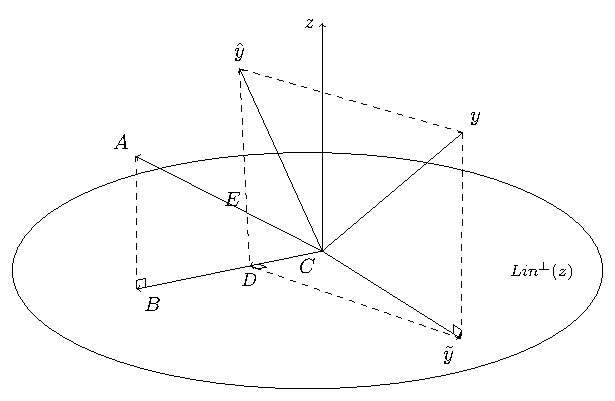
\includegraphics[width=0.45\linewidth]{figures/02_fwl_v2_similar_triangles.pdf}
\label{fig:fwl_v2_triangles}}
\subfigure[]{
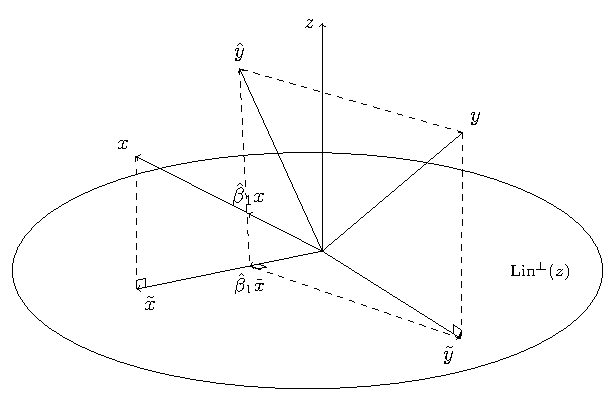
\includegraphics[width=0.45\linewidth]{figures/02_fwl_v2_final.pdf}
\label{fig:fwl_v2_final}}
\caption{\subref{fig:fwl_2_regression_first}: Similar triangles: $\bigtriangleup ABC \sim \bigtriangleup EDC$;
\subref{fig:fwl_2_regression_trans}: Alternative proof for the Frisch-Waugh-Lovell theorem.}
\end{center}
\end{figure}
\end{proof}


\subsection{Duality of regressors and residuals}

The idea of duality is widely used in mathematics.
The concept is to apply some transformation twice and get the~original object.
For example, if $f(a) = 1/a$:
\[
x \stackrel{f}{\to} \frac{1}{x} \stackrel{f}{\to} \frac{1}{1/x} = x
\]
We show that there is duality between regressors and residuals.

\begin{theorem}
Let $x_i$ be a $n \times 1$ regressor,
$u_i$ — a residual in regression of $x_i$ on all the rest regressors,  $i = 1, \ldots, k$.
Consider a transformation of a vector $v$, $f(v) = v/\lVert v \rVert^2$.
Then applying this transformation on the residuals $u_1, \ldots, u_k$ yields
new regressors $v_1, \ldots, v_k$.
Performing $k$ regressions of each $v_i$ on all the rest regressors and
applying the same transformation to the new residuals results in
the original regressors $x_1, \ldots, x_k$.
\end{theorem}

\begin{proof}

\begin{marginfigure}[-2\baselineskip]
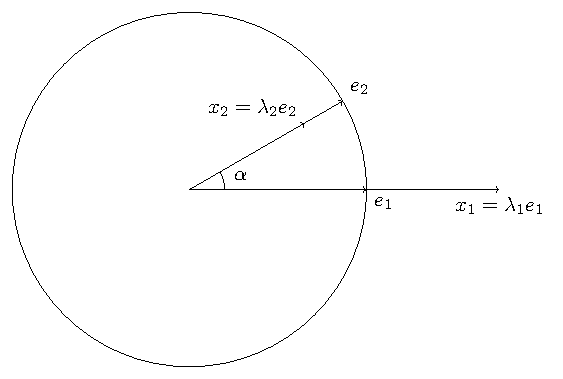
\includegraphics[scale=0.7]{figures/02_duality_original_regressors.pdf}
\caption{Two regressors in the unit circle.}
\end{marginfigure}

We start with $2$-dimensional case with two regressors,
and discuss the~case of spaces of higher dimensions later.

As stated in the~theorem we need to keep the~measure of the~lengths of the~regressors.
In order to do this we choose a~basis in $\mathbb{R}^2$ in such a~way that
\begin{align*}
&x_1 = \lambda_1 e_1, \quad \lVert e_1 \rVert = 1 \\
&x_2 = \lambda_2 e_2, \quad \lVert e_2 \rVert = 1
\end{align*}
where $\lambda_1, \lambda_2 \in \mathbb{R}$.

\begin{marginfigure}
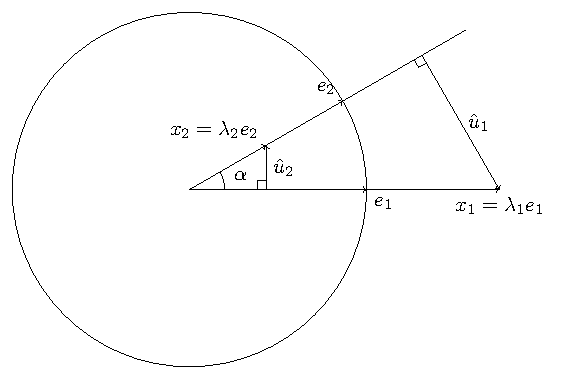
\includegraphics[scale=0.7]{figures/02_duality_first_residuals.pdf}
\label{fig:duality_fst_residuals}
\caption{Residuals $\hat{u}_1$ and $\hat{u}_2$}
\end{marginfigure}

Then we perform two regressions
\begin{align*}
&x_1 = \beta_1 x_2 + u_1 \\
&x_2 = \beta_2 x_1 + u_2
\end{align*}
and get the residuals $\hat{u}_1$, $\hat{u}_2$.
Being orthogonal to $x_2$ and $x_1$, correspondingly, they can be written as follows
\begin{align*}
&\hat{u}_1 = \sin \alpha \cdot \lambda_1 \tilde{e}_1, \quad \lVert \tilde{e}_1 \rVert = 1 \\
&\hat{u}_2 = \sin \alpha \cdot \lambda_2 \tilde{e}_2, \quad \lVert \tilde{e}_2 \rVert = 1
\end{align*}
where $\tilde{e}_1 \perp e_2$ and $\tilde{e}_2 \perp e_1$.

For convenience we translate all the vectors $x_1$, $x_2$, $\hat{u}_1$, $\hat{u}_2$
to the origin of the unit circle as shown in Figure~\ref{fig:duality_fst_residuals_translated}
and after that we invert them.

\begin{marginfigure}
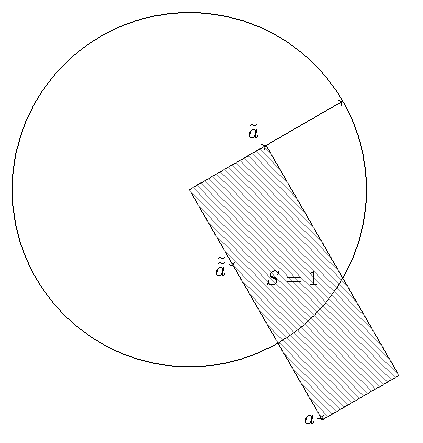
\includegraphics[scale=0.7]{figures/02_duality_inversion.pdf}
\label{fig:duality_inversion}
\caption{Example of inversion for vector $a$.}
\end{marginfigure}

In order to illustrate inversion consider an example with an arbitrary vector $a$.
Knowing its length, the aim is to find such an orthogonal vector $\tilde a$
that the product $\lVert a \rVert^2 \cdot \lVert \tilde a \rVert^2 = 1$.
In other words, we need to find an edge of rectangle with area equal to $1$.
Solving for $\tilde a$, we obtain the length of the inverted vector $a$.
The only thing left is to rotate this inverted vector back
to get a vector $\tilde{\tilde a}$ which satisfies both
\begin{align*}
& \lVert \tilde{\tilde a} \rVert^2 = \frac{1}{\lVert a \rVert^2} \\
& \cos(a, \tilde{\tilde a}) = 1
\end{align*}

\marginnote[-2\baselineskip]{
The transformation stated in the theorem is $f(v) = v / \lVert v \rVert^2$.
Generally speaking, $g(v) = v / (c \cdot \lVert v \rVert^2)$ where $c \in \mathbb{R}$
would also work.
\begin{multline*}
v \stackrel{g}{\to} \frac{v}{c \cdot \lVert v \rVert^2} = w \stackrel{g}{\to} \\
\frac{w}{c \cdot \lVert w \rVert^2} = \frac{\frac{v}{c \cdot \lVert v \rVert^2}}{c \frac{\lVert v \rVert^2}{c^2 \lVert v \rVert^4}} = v
\end{multline*}
}

Having applied the inversion to $\hat{u}_1$, $\hat{u}_2$, we obtained
new vectors $y_1$, $y_2$. Moreover, there is an algebraic expression for them
in terms of rotated basis $\tilde{e}_1$, $\tilde{e}_2$:
\begin{align*}
&\hat{u}_1 = \sin \alpha \cdot \lambda_1 \tilde{e}_1 \Rightarrow y_1 = \frac{1}{\sin \alpha \cdot \lambda_1} \tilde{e}_1 \\
&\hat{u}_2 = \sin \alpha \cdot \lambda_2 \tilde{e}_2 \Rightarrow y_2 = \frac{1}{\sin \alpha \cdot \lambda_2} \tilde{e}_2 \\
\end{align*}

Next, we perform another two regressions:
\begin{align*}
& y_1 = \gamma_1 y_2 + v_1 \\
& y_1 = \gamma_2 y_1 + v_2
\end{align*}

\begin{figure*}[ht!]
\begin{center}
\subfigure[]{
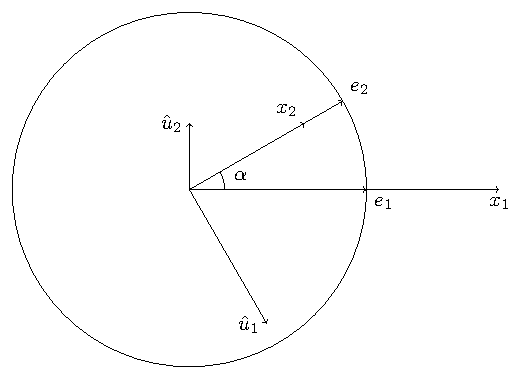
\includegraphics[width=0.3\linewidth]{figures/02_duality_first_residuals_translated.pdf}
\label{fig:duality_fst_residuals_translated}}
\subfigure[]{
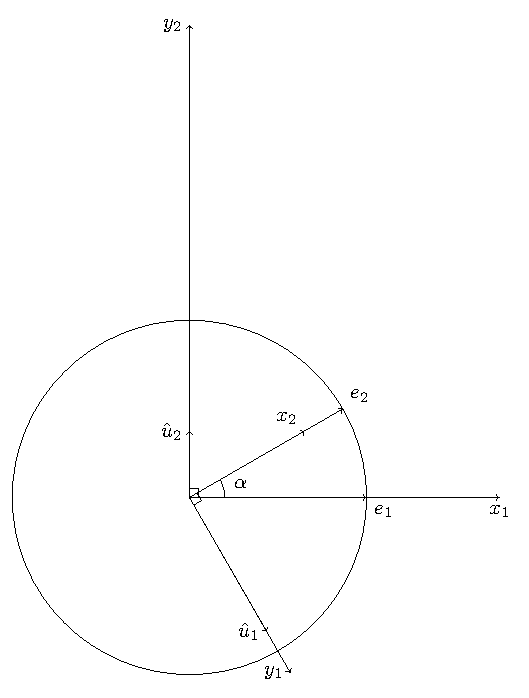
\includegraphics[width=0.3\linewidth]{figures/02_duality_new_regressors.pdf}
\label{fig:duality_new_regreesors}}
\subfigure[]{
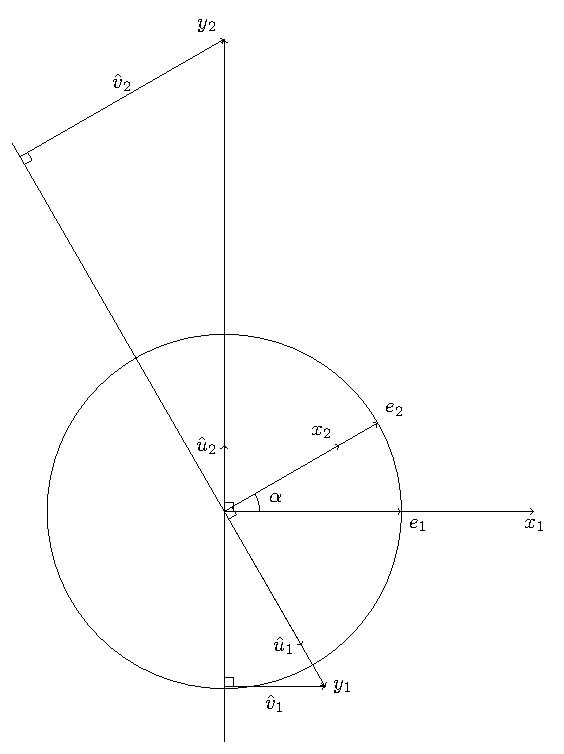
\includegraphics[width=0.3\linewidth]{figures/02_duality_new_residuals.pdf}
\label{fig:duality_new_residuals}}
\caption{\subref{fig:duality_fst_residuals_translated}: Residuals translated to the orgin of the unit circle;
\subref{fig:duality_new_regreesors}: Regressors $v_1$, $v_2$ obtained from inversion of the residuals $\hat{u}_1$, $\hat{u}_2$;
\subref{fig:duality_new_residuals}: Regressions of $v_1$ onto $v_2$ and of $v_2$ onto $v_1$.}
\end{center}
\end{figure*}

There are two things to notice about the new residuals $\hat{v}_1$, $\hat{v}_2$.
First, $\hat{v}_1$ is perpendicular to the line spanned by $\tilde{e}_2$.
Similarly, $\hat{v}_2$ is perpendicular to the line spanned by $\tilde{e}_1$.
This means, that they are parallel to $e_1$, $e_2$, correspondingly,
and once translated, they can be expressed as a multiple of $x_1$, $x_2$.

Second, we can find the lengths of these new residuals from the~right
triangles depicted in Figure~\ref{fig:duality_new_residuals}:
\begin{align*}
& \lVert \hat{v}_1 \rVert = \sin \alpha \cdot \lVert y_2 \rVert = \sin \alpha \cdot \left\lVert \frac{1}{\sin \alpha \cdot \lambda_1} \tilde{e}_1 \right\rVert = \frac{1}{\lambda_1} \\
& \lVert \hat{v}_2 \rVert = \sin \alpha \cdot \lVert y_1 \rVert = \sin \alpha \cdot \left\lVert \frac{1}{\sin \alpha \cdot \lambda_2} \tilde{e}_2 \right\rVert = \frac{1}{\lambda_2}
\end{align*}
Thus, when translated to the origin, the new resiuduals can be rewritten as
\begin{align*}
& \hat{v}_1 = \frac{1}{\lambda_1} e_1 \\
& \hat{v}_2 = \frac{1}{\lambda_2} e_2
\end{align*}

\begin{marginfigure}[20\baselineskip]
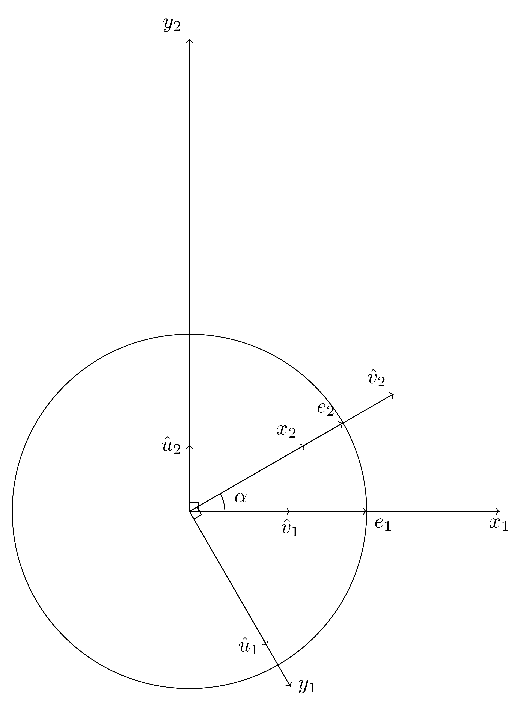
\includegraphics[scale=0.6]{figures/02_duality_final.pdf}
\label{fig:duality_final}
\caption{New residuals translated to the origin of the unit circle.}
\end{marginfigure}

The last step is to invert $\hat{v}_1$, $\hat{v}_2$.
Following the same procedure as described above, we finally get the desired result:
\begin{align*}
& \hat{v}_1 = \frac{1}{\lambda_1} e_1 \to \lambda_1 e_1 = x_1 \\
& \hat{v}_2 = \frac{1}{\lambda_2} e_2 \to \lambda_2 e_2 = x_2
\end{align*}
\end{proof}

\vspace{4cm}
\subsection{Gauss-Markov theorem}

% Hansen
\marginnote{
Consider an estimator $\beta$ which is a linear function of $Y$:
\[
\hat \beta = A^T Y
\]
where $A$ is an $n \times k$ function of $X$ such that $A^T X = I_k$.
From
\begin{align*}
\Var(\hat\beta_{OLS}) &= (X^T X)^{-1} \sigma^2 \\
\Var(A^T y) &= A^T A \sigma^2
\end{align*}
it follows that it is sufficient to prove that $A^T A - (X^T X)^{-1}$
is positive semi-definite. Set $C = A - X(X^T X)^{-1}$ and note that $X^T C = 0$, then
\begin{multline*}
A^T A - (X^T X)^{-1} \\
= (C + X(X^T X)^{-1})^T (C + X(X^T X)^{-1}) - (X^T X)^{-1} \\
= C^T C + C^T X(X^T X)^{-1} + (X^T X)^{-1} X^T C + \\
(X^T X)^{-1} X^T X(X^T X)^{-1} - (X^T X)^{-1} \\
= C^T C
\end{multline*}
Matrix $C^T C$ is positive semi-definite since
\[
\forall a \not= 0 \qquad a^T C^T C a = \lVert C a \rVert^2 \geq 0
\]
}

\begin{theorem}
In the homoskedastic linear regression model the best (minimum-variance) linear
unbiased estimator is given by the ordinary least squares.
\end{theorem}

\begin{proof}
Consider an OLS estimator and an alternative one:
\begin{align*}
\hat{\beta}_{OLS} &= (X^T X)^{-1} X^T y = A^T y \\
\hat{\beta}_{alt} &= A^T_{alt} y
\end{align*}
Note that $A^T X = I_{k}$, then the following holds for all $\beta$:
\begin{align*}
A^T X \beta &= \beta \\
A^T_{alt} X \beta &= \beta
\end{align*}
Taking the difference of these equations, we obtain:
\[
\left(A^T_{alt} - A^T\right) X \beta = 0 \Rightarrow \left(A^T_{alt} - A^T\right) \perp X
\]
If we treat the coefficients separately and consider, for instance, $\beta^{(2)}$,
we get the following result
\[
\left({a^{(2)}}^T_{alt} - {a^{(2)}}^T\right) \perp X
\]
where $a^{(2)}_{alt}$ and $a^{(2)}$ are the second columns of matrices
$A_{alt}$ and $A$ correspondingly.
Since $a^{(2)} \in \Lin(\col X)$, it follows that $a^{(2)}_{alt} \not \in \Lin(\col X)$.

\begin{marginfigure}[1\baselineskip]
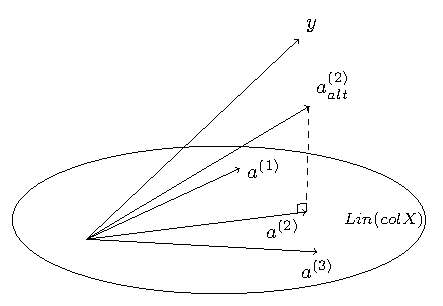
\includegraphics[scale=0.7]{figures/02_gmt.pdf}
\label{fig:gmt}
\caption{Gauss-Markov theorem for the case of three regressors.}
\end{marginfigure}

Now we can express the variances of both estimators in terms of $a^{(2)}_{alt}$ and $a^{(2)}$:
\begin{align*}
\Var\left(\hat{\beta}^{(2)}_{OLS}\right) &= \Var\left({a^{(2)}}^T y\right) = {a^{(2)}}^T \sigma^2 I_{k} a^{(2)} = \sigma^2 \left\lVert a^{(2)} \right\rVert^2 \\
\Var\left(\hat{\beta}^{(2)}_{alt}\right) &= \Var\left({a^{(2)}}^T_{alt} y\right) =  {a^{(2)}}^T_{alt} \sigma^2 I_{k} a^{(2)}_{alt} = \sigma^2 \left\lVert a_{alt}^{(2)} \right\rVert^2
\end{align*}
Since vectors $a^{(2)}$, $a^{(2)}_{alt}$ and $a^{(2)} - a^{(2)}_{alt}$
form a right triangle and $a^{(2)}_{alt} \not \in \Lin(\col X)$,
the vector $\left\lVert a_{alt}^{(2)} \right\rVert^2$ must be longer than $a^{(2)}$,
and the corresponding estimator must have higher variance.

\end{proof}

\subsection{Geometry of instrumental variables}

Consifder a model with an endogenity problem, i.e. explanotary variable $x$
is correlated with the error term $u$:
\[
y = \beta x + u
\]
Assume there is an instrument $z$ which is dependent with the problematic regressor $x$
but uncorrelated with the error term $u$.
The 2SLS procedure tells us to perform the following steps.
\begin{enumerate}
  \item Regress $x$ onto $z$ and get the vector of predicted values $\hat x$,
  \item Regress $y$ onto $\hat x$.
\end{enumerate}
These steps result in $\beta_{IV}$ estimator which is illustrated in Figure~\ref{fig:instrumental}.

The same result could be obtained with the oblique projection.
That is projecting $y$ onto $x$ along the vector perpendicular to the span of $z$.

\begin{marginfigure}
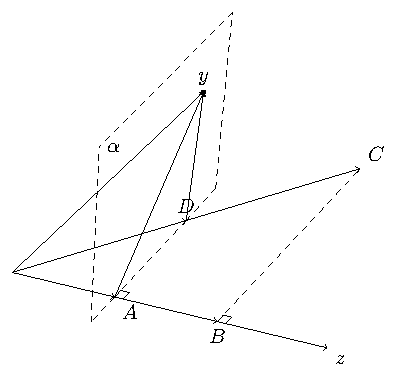
\includegraphics[scale=0.85]{figures/02_instr.pdf}
\caption{Geometry of instrumental variables. $A$ stands for $\hat \beta_{IV} \hat x$,
$B$ — $\hat x$, $C$ — $x$, $D$ — $\hat \beta_{IV} x$.}
\label{fig:instrumental}
\end{marginfigure}

The equivalence of these two methods holds due to the similarity of triangles.
Consider a plane $\alpha$ which satisfies the property of being perpendicular
to the span of $z$, $\alpha \perp z$.
Vectors $x$, $z$ and $\hat x$ form a triangle which is denoted as $\bigtriangleup OBC$
where $\overrightarrow{OB} = \hat{x}$, $\overrightarrow{OC} = x$.
In order to get an oblique projection of $y$ onto $x$ we could either
project $y$ directly onto $x$ staying in the plane $\alpha$
or get the same result in two steps. First, project $y$ onto $z$
and then project the result onto $x$ which gives the same outcome
by the theorem of three perpendiculars. Thus, we get another triangle $\bigtriangleup OAD$
where $\overrightarrow{OA} = \hat \beta_{IV} \hat x$, $\overrightarrow{OD} = \hat \gamma x$.
Since triangles $\bigtriangleup OBC$ and $\bigtriangleup OAD$ are similar
it follows that $\frac{OD}{OC} = \frac{OA}{OB}$ which means that $\hat \gamma = \hat \beta_{IV}$.


\subsection{Geometry of proxy variables}

Consider a model
\[
y = \beta_1 x + \beta_2 w + u
\]
where the error term $u$ is not correlated with the regressors.
Suppose that $w$ is an unobservable variable.
One way to deal with this problem and get a consistent estimator of $\beta_1$ is to use a proxy variable.
In order to clearly state its properties we decompose the unobservable variable
into a sum of a multiple of the proxy ($pr$) and a part that is uncorrelated
with the proxy ($\hat \nu$):
\[
\hat w = \gamma \cdot pr + \hat \nu
\]
Then the proxy variable must satisfy the following properties.
\begin{enumerate}
  \item It must be correlated with the unobservable variable $w$, $pr \not\perp w$.
  \item The error term $\hat u$ must be uncorrelated with the proxy variable, $pr \perp \hat u$.
  \item The error term $\hat \nu$ must be uncorrelated with the regressor $x$, $x \perp \hat \nu$.
\end{enumerate}

\begin{marginfigure}
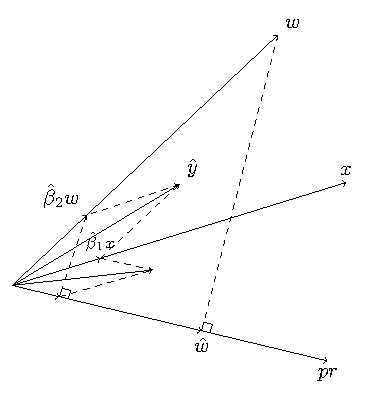
\includegraphics[scale=0.85]{figures/02_proxy.pdf}
\caption{Geometry of proxy variables. }
\label{fig:proxy}
\end{marginfigure}

To get a consistent estimator of $\beta_1$ we need to regress $y$ onto $x$ and $pr$.
Consistency is illustarted in Figure~\ref{fig:proxy}.
Suppose we could get the $\hat y$ by performing the original regression of
$y$ onto $x$ and $w$. Then, $\hat y$ could be decomposed in a sum of
$\hat \beta_1 x$ and $\hat \beta_2 w$.
Notice, that $\hat y$ is both projection of $y$ onto $w$, $x$ and
onto $w$, $x$, $pr$ due to the property of $\hat \nu$ being orthogonal to $x$.
When projected onto the plane spanned by $x$ and $pr$, the $\hat \beta_1 x$
component stays the same as it is already in this plane
while $\hat \beta_2 w$ projects onto the span of $pr$ by the second property of proxy variable.


\newpage
\section{Partial correlations}

\subsection{Definition of a partial correlation}

\marginnote{
A partial correlation is a~measure of the degree of dependence between two random
variables while controlling for the~effect of other random variables:
\[
\pCorr(X,Y; Z) = \frac{\pCov(X,Y;Z)}{\sqrt{\pVar(X;Z)\pVar(Y;Z)}}
\]
where $\pVar(X;Z) = \Var(X - \alpha Z)$, $\alpha$ is such a~constant that $\Cov(X - \alpha Z, Z) = 0$,
and $\pCov(X,Y; Z) = \Cov(X - \alpha Z, Y - \beta Z)$, $\alpha$, $\beta$ are such
constants that $\Cov(X - \alpha Z, Z) = \Cov(Y - \beta Z, Z) = 0$.
}

A partial correlation can be defined in two ways.
We will provide both definitions and show their equivalence.

\begin{definition}
A partial correlation between random variables $X$ and $Y$ holding random variable $Z$
fixed is the~correlation coefficient between the~residuals in regression of $X$ onto
$Z$ and the~residuals in regression of $Y$ onto $Z$.
\end{definition}

Firstly, we project a random variable $X$ onto $Z$, which yields $\E(X \vert Z)$.
The residuals in this regression are $X - \E(X \vert Z)$ — a vector in $\Lin^{\perp}(Z)$.
We will call this variable `cleansed' and label it as $\widetilde X$.
Applying the same procedure for $Y$ yields the `cleansed' variable $\tilde Y = Y - \E(Y \vert Z) \in \Lin^{\perp}(Z)$.
The~angle between $\widetilde X$ and $\widetilde Y$ ($\varphi$ in Figure~\ref{fig:pcorr_def1})
is the~correlation coefficient between these `cleansed' random variables and
the~partial correlation between the~original ones.

\begin{figure}
\centering
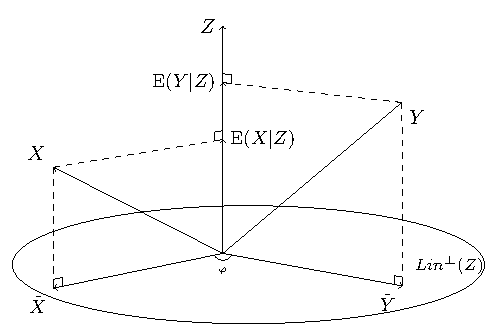
\includegraphics[width=0.55\linewidth]{figures/03_partial_correlation_definition.pdf}
\caption{Partial correlation between $X$ and $Y$ while $Z$ is fixed.}
\label{fig:pcorr_def1}
\end{figure}

\marginnote{
Let us define $\widetilde X$ and $\widetilde Y$ as
\begin{align*}
\widetilde X &= \alpha_{XY} \widetilde Y + \tilde{u}_{XY}, \widetilde X \perp Z \\
\widetilde Y &= \alpha_{YX} \widetilde X + \tilde{u}_{YX}, \widetilde Y \perp Z
\end{align*}
Then assuming that the~error term $u_{XY}$ is uncorrelated with $\widetilde Y$,
we obtain:
\begin{align*}
&\Cov(\widetilde Y, \widetilde X - \alpha_{XY} \widetilde Y) = 0 \\
&\Cov(\widetilde Y, \widetilde X) - \alpha_{XY} \Cov(\widetilde Y, \widetilde Y) = 0 \\
&\alpha_{XY} = \frac{\Cov(\widetilde Y, \widetilde X)}{\Var(\widetilde Y)}
\end{align*}
In the same manner we get $\alpha_{YX}$:
\[
\alpha_{YX} = \frac{\Cov(\widetilde Y, \widetilde X)}{\Var(\widetilde X)}
\]
Note, that $\alpha_{XY}$ and $\alpha_{XY}$ are of the~same sign.
}

\begin{definition}
A partial correlation between random variables $X$ and $Y$ holding random variable $Z$
fixed is the~geometric mean between the coefficient $\beta_{XY}$ in regression
\[
X = \beta_{XY} Y + \beta_{XZ} Z + u_X
\]
and the~coefficinent $\beta_{YX}$ in regression
\[
Y = \beta_{YX} X + \beta_{YZ} Z + u_Y
\]
The partial correlation has the same sign as the~coefficients $\beta_{XY}$ and $\beta_{YX}$.
\end{definition}

Following the~definition, we need to start with regressing variable $X$ onto
$Y$ and $Z$. Then, the vector we obtain $\hat X = \E(X \vert Y, Z)$
can be broken up into the sum of $\beta_{XY} Y$ and $\beta_{XZ} Z$.
Projecting $\beta_{XY} Y$ onto $\Lin^{\perp}(Z)$ results in a~vector
$\alpha_{XY} \widetilde Y$ where $\widetilde Y = Y - \E(Y \vert Z)$
is the projection of $Y$ onto $\Lin^{\perp}(Z)$.

\marginnote{
Multiplying these coefficients, we get the final result:
\begin{multline*}
\alpha_{XY} \cdot \alpha_{XY} = \frac{\Cov^2(\widetilde Y, \widetilde X)}{\Var(\widetilde Y)\Var)\widetilde X} \\
= \Corr^2(\widetilde X, \widetilde Y) = \pCorr^2(X,Y; Z)
\end{multline*}
}

By the~properties of similar triangles
\[
\frac{\beta_{XY} Y}{Y} = \frac{\alpha_{XY} \widetilde Y}{\widetilde Y} \Leftrightarrow \beta_{XY} = \alpha_{XY}
\]

In the same way we perform a regression of $Y$ onto $X$ and $Z$ and repeat the
same steps for $X$. Finally, we get the whole picture:

\begin{figure}[ht!]
\begin{center}
\subfigure[]{
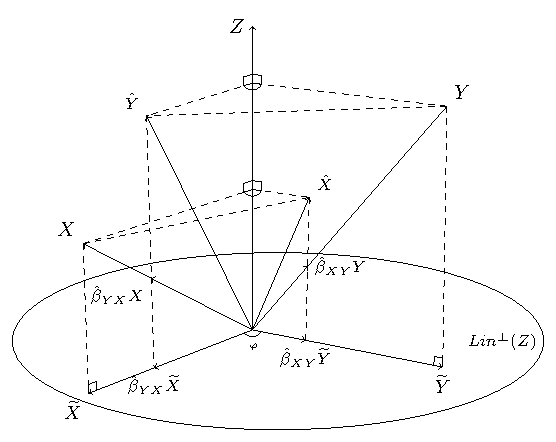
\includegraphics[width=0.55\linewidth]{figures/03_partial_correlation_regression_definition.pdf}
\label{fig:part_corr_alt}}
\subfigure[]{
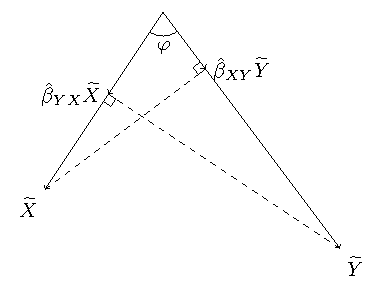
\includegraphics[width=0.35\linewidth]{figures/03_partial_correlation_regression_definition_lin.pdf}
\label{fig:part_corr_alt_lin}}
\caption{\subref{fig:part_corr_alt}: Alternative definition of the partial correlation;
\subref{fig:part_corr_alt_lin}: $\Lin^{\perp}(Z)$.}
\end{center}
\end{figure}

Having plotted $\Lin^{\perp}(Z)$, now we can express $\cos \varphi$ in terms of $\beta_{XY}$
and $\beta_{YX}$. We use the fact that $\beta_{XY} \beta_{YX} > 0$:

\begin{equation*}%\label{eq:part_cor_cos}
\begin{split}
\cos \varphi &= \frac{\vert \beta_{XY} \widetilde Y \vert}{\vert \widetilde X \vert} \\
\cos \varphi &= \frac{\vert \beta_{YX} \widetilde X \vert}{\vert \widetilde Y \vert} \\
\cos^2 \varphi &= \vert \beta_{XY} \beta_{YX} \vert \stackrel{\beta_{XY} \beta_{YX} > 0}{=} \beta_{XY} \beta_{YX}
\end{split}
\end{equation*}

Recall that the angle $\varphi$ can be interpreted as the correlation
between $\widetilde X$ and $\widetilde Y$.
These random variables are constructed in such a way that both of them
are uncorrelated with $Z$. Thus, it follows that
\[
\cos^2 \varphi = \Corr^2(\widetilde X, \widetilde Y) = \pCorr^2(X,Y; Z) = \beta_{XY} \beta_{YX}
\]

\subsection{Partial correlation as correlation between residuals}

\marginnote{
Let us define cleansed $X$ and $Y$ first as
\begin{align*}
\widetilde{X} &= \alpha_1 \widetilde{Y} + \tilde{u}, \widetilde{X} \perp Z \\
\widetilde{Y} &= \beta_1 \widetilde{X} + \tilde{v}, \widetilde{Y} \perp Z
\end{align*}
Then
\begin{align*}
\alpha_1 &= \frac{\Cov(\widetilde{X}, \widetilde{Y})}{\Var(\widetilde{Y})} \\
\beta_1 &= \frac{\Cov(\widetilde{X}, \widetilde{Y})}{\Var(\widetilde{X})}
\end{align*}
}



\begin{theorem}
The partial correlation between $X$ and $Y$ holding $Z$ fixed is the negative
correlation coefficient between the residuals $u$ in the regression model
\[
X = \alpha_1 Y + \alpha_2 Z + u
\]
and the residuals $v$ in the model
\[
Y = \beta_1 X + \beta_2 Z + v
\]
\end{theorem}

\begin{proof}
The first step is to find the residuals in the regressions.
For example, in order to get $u$ we regress $X$ onto $\Lin(Y,Z)$
which results in $\hat X = X - \E(X \vert Y, Z)$.
Then we take the difference $X - \hat X = u$
and project it and $X$ itself onto $\Lin^{\perp}(Z)$ as demonstrated
in Figure~\ref{fig:pcorr_t_x}.
We denote the result as $\tilde u$ and $\widetilde X$ respectively.

Figure~\ref{fig:pcorr_t_y} shows the same steps for obtaining $\tilde v$ and $\widetilde Y$.

\marginnote[-6\baselineskip]{
Substituting these into $\Cov(\tilde{u}, \tilde{v})$, we obtain:
\begin{align*}
&\Cov(\tilde{u}, \tilde{v}) = \\
&\Cov\left(\widetilde{X} - \frac{\Cov(\widetilde{X}, \widetilde{Y})}{\Var(\widetilde{Y})} \widetilde{Y},
\widetilde{Y} -  \frac{\Cov(\widetilde{X}, \widetilde{Y})}{\Var(\widetilde{X})} \widetilde{X}\right) \\
&= \Cov(\widetilde{X}, \widetilde{Y}) - \Cov(\widetilde{X}, \widetilde{Y}) \\
&- \Cov(\widetilde{X}, \widetilde{Y}) + \frac{\Cov^3(\widetilde{X}, \widetilde{Y})}{\Var(\widetilde{X})\Var(\widetilde{Y})} \\
&= - \Cov(\widetilde{X}, \widetilde{Y}) \left(1 - \frac{\Cov^2(\widetilde{X}, \widetilde{Y})}{\Var(\widetilde{X})\Var(\widetilde{Y})} \right)
\end{align*}
Next, we deal with variances of $\tilde{u}$ and $\tilde{v}$:
\begin{align*}
\Var(\tilde{u}) &= \Var(\widetilde{X}) - \frac{\Cov^2(\widetilde{X}, \widetilde{Y})}{\Var^2(\widetilde{Y})} \Var(\widetilde{Y}) \\
&- 2 \Cov(\widetilde{X}, \widetilde{Y}) \frac{\Cov(\widetilde{X}, \widetilde{Y})}{\Var(\widetilde{Y})} \\
&= \Var(\widetilde{X}) \left(1 - \frac{\Cov^2(\widetilde{X}, \widetilde{Y}}{\Var(\widetilde{X}) \Var(\widetilde{Y})}\right) \\
&\Var(\tilde{v}) = \Var(\widetilde{Y}) \left(1 - \frac{\Cov^2(\widetilde{X}, \widetilde{Y}}{\Var(\widetilde{X}) \Var(\widetilde{Y})}\right)
\end{align*}
Now we can write out $\Corr(\tilde{u}, \tilde{v})$:
\begin{align*}
&\Corr(\tilde{u}, \tilde{v}) = \\
&= -\frac{\Cov(\widetilde{X}, \widetilde{Y}) \left(1 - \frac{\Cov^2(\widetilde{X}, \widetilde{Y})}{\Var(\widetilde{X})\Var(\widetilde{Y})} \right)}{\sqrt{\Var(\widetilde{X})\Var(\widetilde{Y}) \left(1 - \frac{\Cov^2(\widetilde{X}, \widetilde{Y})}{\Var(\widetilde{X}) \Var(\widetilde{Y})}\right)^2 }} \\
&= -\Corr(\widetilde{X}, \widetilde{Y})
\end{align*}
}

\begin{figure}[ht!]
\begin{center}
\subfigure[]{
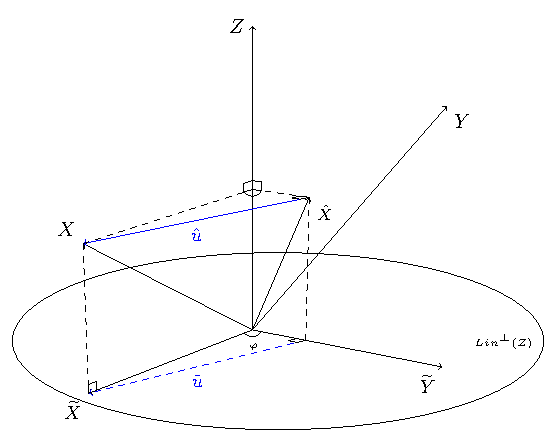
\includegraphics[width=0.45\linewidth]{figures/03_partial_correlation_residuals_x.pdf}
\label{fig:pcorr_t_x}}
\subfigure[]{
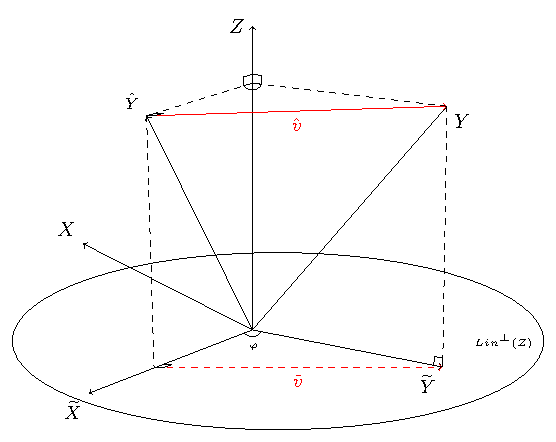
\includegraphics[width=0.45\linewidth]{figures/03_partial_correlation_residuals_y.pdf}
\label{fig:pcorr_t_y}}
\caption{\subref{fig:pcorr_t_x}: $\hat u$ form regression of $X$ onto $Y$ and $Z$, $\hat u$ projected;
\subref{fig:pcorr_t_y}: $\hat v$ from regression of $Y$ onto $X$ and $Z$, $\hat v$ projected.}
\end{center}
\end{figure}


After putting these figures together, we need to measure the angle
between the $\tilde u$ and $\tilde v$.
Translating the $\tilde v$ vector to the orgin of $\tilde x$ as shown in Figure~\ref{fig:pcorr_t_lin},
we conclude that the desired angle is the bigger of the vertical angles.
Hence, we can derive it from the property of the quadrilateral
by substracting all the known angles from $360^\circ$.
Thus, the desired angle is $180^\circ - \varphi$.
\begin{align*}
\cos\varphi &= - \cos(180^\circ - \varphi) \\
\Corr(\widetilde X, \widetilde Y) &= -\Corr(\tilde u, \tilde v) \\
\pCorr(X,Y; Z) &= -\Corr(u, v)
\end{align*}


\begin{figure}[ht!]
\begin{center}
\subfigure[]{
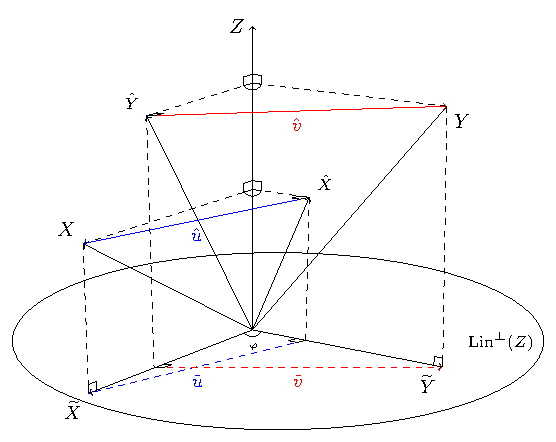
\includegraphics[width=0.45\linewidth]{figures/03_partial_correlation_residuals_xy.pdf}
\label{fig:pcorr_t_xy}}
\subfigure[]{
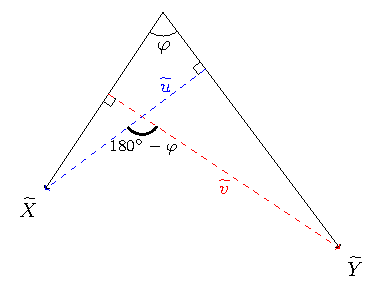
\includegraphics[width=0.45\linewidth]{figures/03_partial_correlation_residuals_xy_lin.pdf}
\label{fig:pcorr_t_lin}}
\caption{\subref{fig:pcorr_t_x}: The residuals of both regressions;
\subref{fig:pcorr_t_y}: $\Lin^{\perp}(Z)$.}
\setfloatalignment{b}
\end{center}
\end{figure}
\end{proof}


\newpage
\section{Probability distributions}

\subsection{Normal}

By contrast with substantial majority of books, the univariate normal distribution
can be derived form the multivariate normal distribution.
In this section we show how to obtain the univariate normal from the bivariate.

\begin{marginfigure}
  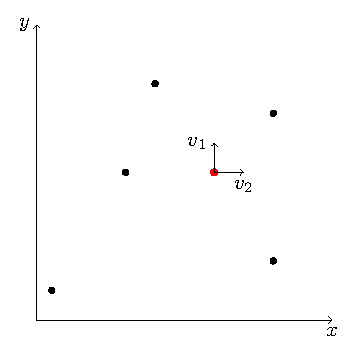
\includegraphics[width=\linewidth]{figures/04_normal.pdf}
  \caption{Black dots represent the gas molecules.
  The red dot stands for the one we catch.
  Its speed along the horizontal axis is $v_1$, i.e., the first component of
  the velocity vector, and its speed along the vertical axis is $v_2$.}
\end{marginfigure}

The original idea belongs to J.C. Maxwell who was wondering
what distribution the velocity of gas molecules follow.
The similar question was also bothering J.H.W. Herschel who was an astronomer
and was dealing with measurement errors in astronomical data.
Here we provide a proof of the theorem known today as Herschel-Maxwell's.

Assume there are gas molecules moving chaotically on a plane
and we can measure the velocity vector of one of them.
We will denote this vector as $V = \begin{pmatrix} X \\ Y \end{pmatrix}$
where $X$ and $Y$ stand for the horizontal and vertical components respectively.
Assume additionally that
\begin{enumerate}
  \item The joint distribution finction $f(x,y)$ does not depend on
  the vector $(X,Y)^T$ direction but depends on its length only;
  \item The orthogonal components of the velocity vector are independent;
  \item And we measure the velocity in such a way that $\Var(X) = 1$.
\end{enumerate}

\marginnote{
It is more common to introduce a standard normal distribution in terms of its PDF
\begin{definition}
A continuous random variable $\xi$ has a standard normal distribution
if its PMF is given by
\[
f_{\xi} (x) = \frac{1}{\sqrt{2\pi}}\exp\left(-\frac{x^2}{2}\right).
\]
\end{definition}
After that multivariate normal is defined.

\begin{definition}
Let $\xi_i \stackrel{iid}{\sim} \mathcal{N}(0, 1)$ then $\xi \sim \mathcal{N}(\vec{0}, I)$
where $\xi = \begin{pmatrix} \xi_1 \\ \vdots \\ \xi_n \end{pmatrix}$,
$I$ is $n \times n$ identity matrix, and its PMF is
\[
f_{\xi} (x_1, \ldots, x_n) = \frac{1}{(\sqrt{2\pi})^n}\exp\left(-\frac{x_1^2+\ldots+x_n^2}{2}\right).
\]
\end{definition}
And finally, location-scale transformations are applied.
}

\begin{theorem}
Assumptions (1) and (2) are satisfied if and only if
$X \sim \mathcal{N}(0, \sigma^2)$, $Y \sim \mathcal{N}(0, \sigma^2)$
and $X$, $Y$ are independent.
\end{theorem}

\begin{proof}
First of all, consider a vector $V' = \begin{pmatrix} -Y \\ X \end{pmatrix}$, i.e.,
the original vector $V$ rotated $90^{\circ}$ counterclock-wise.
By the assumption (1), this operation did not change the distribution of $V$.
Hence, $V' \sim V$ which implies $-Y \sim X$ and $X \sim Y$.
It follows that
\[
\begin{cases}
\E(-Y) = \E(X) \\
\E(X) = \E(Y)
\end{cases}
\]
which holds for $\E(X) = \E(Y) = 0$ only.
However, we have to notice that $\E(X)$ may not exist at all.

Likewise, $\Var(X) = \Var(Y)$ and it follows from the assumption (3)
that $\Var(X) = \Var(Y) = 1$.

Next, we introduce the angle between $V$ and the horizontal axis $U$ and
the length of the velocity vector $R = \sqrt{X^2 + Y^2}$.
Obviously, $X = R \cos U$ and $Y = R \sin U$.
Note that since the joint distribution of $X$ and $Y$ depends only on
the length of vector $V$ the distribution function of $U$ can only be constant,
thus $U \sim Unif(0, 2\pi)$.

Applying assumption (1) again, we conclude that the joint distribution function
can be written as a function of the length of the velocity vector, or equivalently
of the length squared:
\[
f(x,y) = h(x^2 + y^2).
\]
By the assumption (2), orthogonal components of $V$ are independent.
Hence, the joint PMF can be decomposed to the product of marginal ones:
\[
f(x,y) = f(x)f(y) = g(x^2)g(y^2)
\]
where the latter equality was written for convenience.
Putting everything together, we obtain
\[
h(x^2 + y^2) = g(x^2)g(y^2).
\]
Next, we take the derivative of both sides with respect to $y^2$ and
then substitute $y^2 = 0$ to get a constant $k$:
\begin{align*}
h'(x^2 + y^2) &= g(x^2)g'(y^2) \\
h'(x^2) &= g(x^2)g'(0) \\
h'(x^2) &= k \cdot g(x^2)
\end{align*}

\marginnote{
In order to obtain $k$ we computed
\begin{align*}
\E(X^2) &= \int_{-\infty}^{\infty} x^2 \sqrt{c} e^{kx^2} dx \\
&= \left. x \cdot \sqrt{c} e^{kx^2} \cdot \frac{k}{2} \right|_{-\infty}^{\infty} - \int_{-\infty}^{\infty} \sqrt{c} e^{kx^2} \cdot \frac{1}{2k} dx \\
&= - \frac{1}{2k} \int_{-\infty}^{\infty} \sqrt{c} e^{kx^2} \\
&= - \frac{1}{2k} \cdot 1 \\
&= 1.
\end{align*}
}

Solving the differential equation, we obtain
\[
h(x^2) = c e^{kx^2}, \quad c \in \mathbb{R}.
\]
So the joint PMF can be written as follows:
\[
f(x,y) = h(x^2 + y^2) = c e^{k(x^2+y^2}
\]
and due to independece of $X$ and $Y$ the PMF of $X$ is
\[
f(x) = \sqrt{c} e^{kx^2}.
\]

\marginnote{
In order to obtain $c$ we computed:
\begin{align*}
\int_{-\infty}^{\infty} \int_{-\infty}^{\infty} e^{-\frac{x^2 + y^2}{2}} dx dy &= \int_{0}^{2\pi} \int_{0}^{\infty} e^{-\frac{r^2}{2}}r dr d\theta \\
&= \int_{0}^{2\pi} \left(\int_{0}^{\infty} e^{-u} du \right) d\theta \\
&= \int_{0}^{2\pi} 1 d\theta \\
&= 2 \pi.
\end{align*}
}

In order to find the constant $k$, we need to solve $\E(X^2) = 1$.
Computing the integral we obtain $k=-\frac{1}{2}$.

Finally, we need to normalize $f(x) = c e^{-\frac{x^2 + y^2}{2}}$ so as to
obtain $c$. Again, computing another integral,
we conclude that $c=(2\pi)^{-1}$ which finishes the proof.
\end{proof}

Notice, that any other $\mathcal{N}(\mu, \sigma^2)$ can be obtained by applying
location-scale transformations.

The theorem can be generalized to the n-dimensional case.
\begin{theorem}\label{th:mvn}
The vector $z = \begin{pmatrix} z_1 \\ \vdots \\ z_n \end{pmatrix}$
follows the standard multivariate normal distribution and its components
are independent if and only if
\begin{enumerate}
  \item f(z) depends on $\vert z \vert$ only,
  \item the projections of vector $z$ onto the orthogonal subspaces $A$ and $B$
  in $\mathbb{R}^n$ are independent.
\end{enumerate}
\end{theorem}


\subsection{Chi-squared}

\marginnote{
\begin{definition}\label{def:chi_traditional}
Let $z_i \stackrel{iid}{\sim} \mathcal{N}(0,1)$.
Then $Q$ follows the chi-squared distribution with $k$ degrees of freedom
if it can be written as
\[
Q = z_1^2 + z_2^2 + \ldots + z_k^2.
\]
\end{definition}

This definition is a particular case of the geometric one.
Consider projecting a vector $z = (z_1, z_2, \ldots, z_n)$ form $\mathbb{R}^n$
onto the~$k$-dimensional subspace $S$ of vectors which first $k$ coordinates
are arbitrary and all the rest are zeros. As a result we would get
\[
\hat z = (z_1, z_2, \ldots, z_k, 0, \ldots, 0).
\]
Squaring the length of the projection, we obtain
\[
Q = \lVert \hat z \rVert = z_1^2 + z_2^2 + \ldots + z_k^2.
\]
}

\begin{definition}\label{th:chi}
Consider a random vector $z \in \mathbb{R}^n$ which components are independent
and follow standard normal distribution, $z_i \sim \mathcal{N}(0,1)$.
Consider also a $k$-dimensional subspace $L$ in $\mathbb{R}^n$.
Let the projection of vector $z$ onto the subspace $L$ be $\hat z$ and
its length squared $Q$
\[
Q = \lVert \hat z \rVert^2 = \langle \hat z, \hat z \rangle = \hat z^T \hat z
\]
Then $Q$ follows the chi-squared distribution with $k$ degrees of freedom.
\end{definition}

\begin{theorem}
The definitions~\ref{def:chi_traditional} and \ref{th:chi} are equivalent.
\end{theorem}

\begin{proof}
First, it can be shown that the~projected vector $\hat z$ is the~original vector $z$
multiplied by the~projection matrix $H = X(X^T X)^{-1}X^T$ where the columns of $X$
are fixed linearly independent vectors $x_1, \ldots, x_k$ in $L$
or equivalently $\col X = \Lin(x_1, \ldots, x_k)$.
This matrix is  also often referred to as `hat-matrix'.
Then the statement in~the~theorem can be rewritten as follows:
\[
\hat z^T \hat z = (Hz)^T Hz = z^T H^T H z = z^T H^2 z = z^T H z,
\]
applying the idempotence property in the last step.

Another nice property of~the~hat-mattix is symmetry.
Thus, it can be decomposed as
\[
H = P D P^T,
\]
where we choose the vectors of matrix $P$ to be unit and orthogonal,
and $D = diag{(\lambda_1, \ldots, \lambda_n)}$ where $\lambda_i$ is an eigenvalue of $H$.

\begin{marginfigure}
  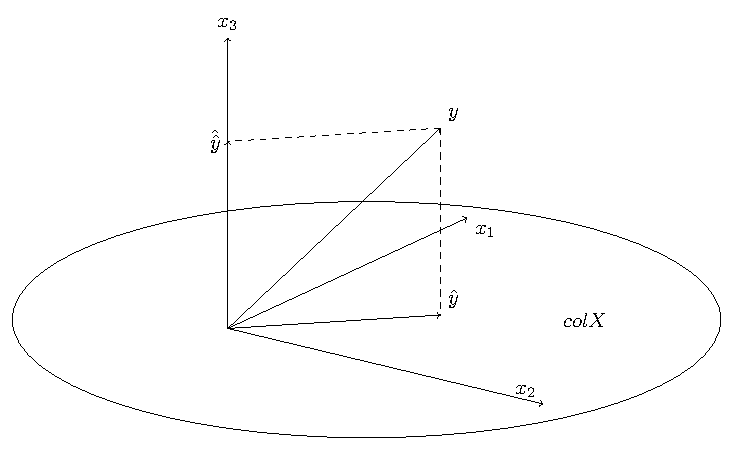
\includegraphics[width=\linewidth]{figures/04_chi_squared_example.pdf}
  \caption{Consider a $3$-dimensional example, $\col X = \Lin(x_1, x_2)$ and $col^{\perp}X = \Lin(x_3)$.
  $H x_1 = x_1$ and $H x_2 = x_2$ since they are in $\col X$. However, $H x_3 = 0$ as $x_3 \perp \col X$.
  Projecting an arbitrary vector onto $\col X$ yileds $Hy = \hat y \in \Lin(x_1, x_2)$
  while projecting onto $col^{\perp}X$ results in $(I-H)y = \hat{\hat y} \in \Lin(x_3)$.}
\end{marginfigure}

Since $H^2 = H$ the eigenvalues are either $0$ or $1$.
Recall that $H$ projects a vector onto $\col X$.
Then for any $x_i$, $i = 1, \ldots, k$, $H x_i = x_i \cdot 1$ since
any $x_i$ is already in $\col X$. This implies that $\lambda_1 = \ldots = \lambda_k = 1$.
There are also $n-k$ vectors in the subspace orthogonal to $\col X$.
So for any $x_i$, $i= k+1, \ldots, n$, the orthogonal projection yields zero.
We conclude that $\lambda_{k+1} = \ldots = \lambda_n = 0$.

Rewritting the theorem statement further, we obtain
\[
z^T H z = z^T P D P^T z = (P^T z)^T D (P^T z) = \tilde z^T D \tilde z = \tilde z_1^2 + \ldots + \tilde z_k^2.
\]
Now we explore $\tilde z$ given $z \sim \mathcal{N}(0, I)$:
\begin{align*}
&\tilde z = P^T z \\
&\E(\tilde z) = \E(P^T z) = P^T \E(z) = 0 \\
&\Var(\tilde z) = \Var(P^T z) = P^T \Var(z) (P^T)^T = P^T P = I
\end{align*}
So we conclude that $\tilde z_1^2 + \ldots + \tilde z_k^2 \sim \chi^2_k$.

\end{proof}


\subsection{Student's}

\marginnote{
A continuous random variable $T$ has Student's distribution with $k$ degrees
of freedom if it can be expressed as
\[
T = \frac{Z}{\gamma_k/\sqrt{k}},
\]
where $Z \sim \mathcal{N}(0,1)$, $\gamma_k \sim \chi^2_{k}$ and
$Z$, $\gamma_k$ are independent.
}

\begin{definition}
Let  $z = \begin{pmatrix} z_1 \\ \vdots \\ z_n \end{pmatrix}$
where $z_i \sim \mathcal{N}(0, \sigma^2), i=1, \ldots, n$ and are independent.
Let $L_1$ be 1-dimensional subspace in $\mathbb{R}^{n}$, $L_2$ an orthogonal to $L_1$ subspace.
Then
\[
T = \frac{\lVert H_1 z \rVert}{\lVert H_2 z \rVert / \sqrt{\dim L_2}}
\]
where $\lVert H_1 z \rVert$ is the length of the projection of vector $z$ onto
1-dimensional subspace $L_1$,
$\lVert H_2 z \rVert$ — the length of the projection onto $L_2$,
follows Student's distribution with $\dim L_2$ degrees of freedom.
\end{definition}

Let us choose two orthogonal subspaces: one-dimensional $L_1$ and
$k$-dimensional $L_2$.

Previously we showed that, the squared length of projection follows
the chi-squared distribution with the degrees of freedom equal to the dimension
onto which the vector was projected. Thus, $\lVert H_1 z \rVert^2 \sim \chi^2_1$
and $\lVert H_2 z \rVert^2 \sim \chi^2_{k}$.
Now we can express $T^2$ as a ratio of the per-dimension lengths squared:
\[
T^2 = \frac{\lVert H_1 z \rVert^2}{\lVert H_2 z \rVert^2 / \dim L_2}
\]
Taking the square root of both sides, we obtain:
\[
T = \frac{\lVert H_1 z \rVert}{\lVert H_2 z \rVert / \sqrt{\dim L_2}} = \tg \varphi
\]
The latter equality can be illustarted with a $3$-dimensional example (see Figure~\ref{fig:f_dist}).





\subsection{t-test}

In a simple linear regression model
\[
y = \beta_1 + \beta_2 x + \varepsilon
\]
the adjusted t-value $\frac{t}{\sqrt{n-2}}$ when $H_0: \beta_2 = 0$ is tested
can be expressed in terms of the angle between $y$ and $\hat y$ $\varphi$ and
is equal to $\ctg \varphi$.

Recall that the t-statistic is defined in the following way:
\[
t = \frac{\hat \beta - \beta}{se\left(\hat\beta\right)}
\]
Adjusting this formula for the null hypothesis $H_0: \beta_2 = 0$, we obtain
\begin{equation}\label{eq:tstat}
t = \frac{\hat \beta_2}{se\left(\hat\beta_2\right)}
\end{equation}
Then, we need to express $se\left(\hat\beta_2\right)$ in terms of vectors which can be
plotted. From standard OLS procedure it follows that
\begin{equation}\label{eq:varbeta2}
\Var(\hat \beta_2) = \frac{\sigma^2}{\sum\limits_{i=1}^n (x_i - \bar x)^2}
\end{equation}
Since actual $\sigma$ is unknown the estimator will be used instead:
\begin{equation}\label{eq:sigmaest}
\hat \sigma^2 = \frac{RSS}{n-2}
\end{equation}
Substituting \eqref{eq:varbeta2} and \eqref{eq:sigmaest} into \eqref{eq:tstat}
divided by $\sqrt{n-2}$, we obtain
\begin{align*}
\frac{t}{\sqrt{n-2}} &= \frac{\hat \beta_2}{\sqrt{n-2}se\left(\hat\beta_2\right)} = \frac{\hat \beta_2}{\sqrt{n-2}\frac{\hat \sigma}{\sqrt{\sum\limits_{i=1}^n (x_i - \bar x)^2}}} \\
&= \frac{\hat \beta_2 \sqrt{\sum\limits_{i=1}^n (x_i - \bar x)^2}}{\sqrt{n-2}\frac{\sqrt{\sum\limits_{i=1}^n (y_i - \hat y_i)^2}}{\sqrt{n-2}}} = \frac{\hat \beta_2 \vert x^c \vert}{\sqrt{RSS}}
\end{align*}
where $ \vert x^c \vert = \sqrt{\sum_{i=1}^n (x_i - \bar x)^2}$ is the length of the
centred vector $x$.

Now the result can be demonstrated visually.
Again we will project $x$ and $y$ vectors onto the $\Lin^{\perp}(\mathbf{1})$ so as to
get their centred versions $x^c$ and $y^c$.
Then, we perform regression of $y$ onto $\Lin(x, \mathbf{1})$ which results in $\hat y$.
Following that, we project $\hat y = \hat \beta_1 + \hat \beta_2 x$ onto $\Lin^{\perp}(\mathbf{1})$
which yields $\hat \beta_2 x^c$.
After all, we translate $\sqrt{RSS}$ onto $\Lin^{\perp}(\mathbf{1})$.
These steps are demonstrated in Figure~\ref{fig:ttest_3d}.

Looking at Figure~\ref{fig:ttest_lin} which depicts the $\Lin^{\perp}(\mathbf{1})$,
we derive
\[
\ctg \varphi = \frac{\hat \beta_2 \vert x^c \vert}{\sqrt{RSS}} = t
\]

\begin{figure}[ht!]
\begin{center}
\subfigure[]{
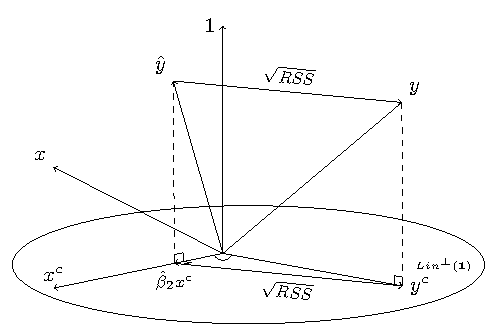
\includegraphics[width=0.45\linewidth]{figures/04_ttest.pdf}
\label{fig:ttest_3d}}
%\hspace{4ex}
\subfigure[]{
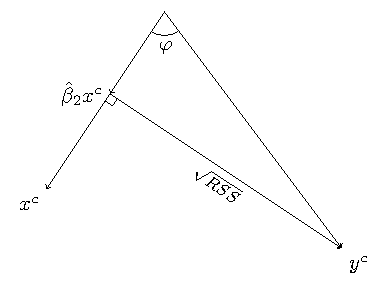
\includegraphics[width=0.45\linewidth]{figures/04_ttest_lin.pdf}
\label{fig:ttest_lin}}
\caption{\subref{fig:pcorr_t_x}: Regression of $y$ onto $\Lin(x, \mathbf{1})$ and appropriate projections;
\subref{fig:pcorr_t_y}: $\Lin^{\perp}(\mathbf{1})$.}
\end{center}
\end{figure}


\subsection{F-distribution}

\marginnote{
Generally, the following definition is given.
\begin{definition}
Let $\gamma_1 \sim \chi^2_{k_1}$, $\gamma_2 \sim \chi^2_{k_2}$,
$\gamma_1$, $\gamma_2$ independent.
Then
\[
\frac{\gamma_1/k_1}{\gamma_2/k_2} \sim F_{k_1, k_2}.
\]
\end{definition}
}

\begin{definition}\label{def:f}
Let $z = \begin{pmatrix} z_1 \\ \vdots \\ z_n \end{pmatrix}$
where $z_i \sim \mathcal{N}(0, \sigma^2)$ and are independent.
Let $L_1$, $L_2$ be orthogonal subspaces in $\mathbb{R}^n$.
then
\[
F = \frac{\lVert H_1 z \rVert^2 / \dim L_1}{\lVert H_2 z \rVert^2 / \dim L_2} \sim F_{\dim L_1, \dim L_2},
\]
where $\lVert H_1 z \rVert^2$, $\lVert H_2 z \rVert^2$ are the squared lengths
of $z$ projected onto $L_1$ and $L_2$ respectively.
\end{definition}

Recall that by Theorem~\ref{th:mvn} the projections of a standard noraml vector
onto orthogonal subspaces are independent.
Thus, in terms of the Definition~\ref{def:f} $H_1 z$ and $H_2 z$ are independent.
Next, from the Definition~\ref{th:chi} where we defined the chi-squared distribution
it follows that the squared lengths of these projections follow
the chi-squared distribution with the number of degrees of freedom
equal to the dimension of the subspace onto which the vector was projected.
In other words, $\lVert H_1 z \rVert^2 \sim \chi^2_{\dim L_1}$,
$\lVert H_2 z \rVert^2 \sim \chi^2_{\dim L_2}$.

\begin{marginfigure}
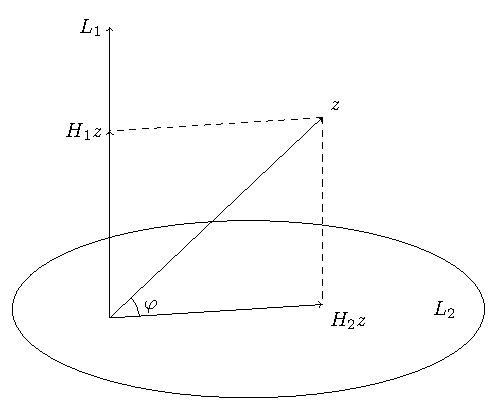
\includegraphics[scale=0.7]{figures/04_f_dist_example.pdf}
\caption{F-distribution as the ratio of the projection lengths squared
adjusted to the dimensions of the subspaces.}
\label{fig:f_dist}
\end{marginfigure}

Taking the ratio of these length squared, we get the interpretaion
of the angle between the original vector $z$ and its projection onto $L_1$:
\[
tg^2 \varphi = \frac{\lVert H_1 z \rVert^2}{\lVert H_2 z \rVert^2}.
\]
Adjusting this ratio to the degrees of freedom, we get the desired definition.


\subsection{F-test}

The significance of several coefficients at once can be tested with the F-test.
The F-statistic has the following form
\[
F = \frac{(RSS_{R} - RSS_{UR})/q}{RSS_{UR}/(n-k_{UR})}
\]
where indices $R$ and $UR$ stand for the restricted and unrestricted models
respectively, $n$ — number of observations, $k$ — number of regressors,
$q$ — number of equtions used in the null hypothesis.

\begin{marginfigure}
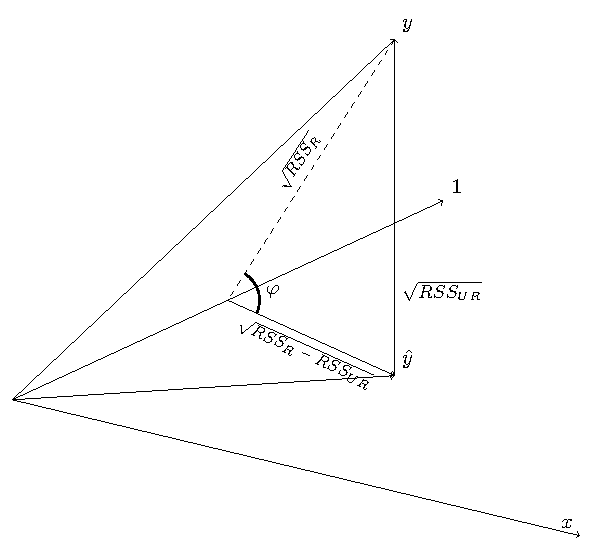
\includegraphics[scale=0.55]{figures/04_ftest.pdf}
\caption{F-statistic as the cotangent squared of $\varphi$
where $a$ stands for $\sqrt{RSS_{UR}}$, $b$ — $\sqrt{RSS_{R} -RSS_{UR}}$,
$c$ — $\sqrt{RSS_{R}}$.}
\label{fig:ftest}
\end{marginfigure}

Due to plotting limitations, we consider the unrestricted model to be
\[
y = \beta_1 + \beta_2 x + u
\]
and the restricted model to be
\[
y = \alpha_1 + v
\]
Note that there was a choice in the restricted models.


We perform both regressions in order to get the ressiduals and plot them
in Figure~\ref{fig:ftest}.
Adjusted to the degrees of freedom, the ratio can be expressed in terms of the
angle between two vectors, $\varphi$, as demonstrated in Figure~\ref{fig:ftest}
\[
F = \frac{(RSS_{R} - RSS_{UR})/q}{RSS_{UR}/(n-k_{UR})} = \ctg^2 \varphi
\]


%\newpage
%\section{Ideas to develop}


\newpage
\printbibliography[
heading=bibintoc,
title={References}
]

\end{document}
